% This document provides the style to be used for a MSc Thesis at the
% Parallel and Distributed Systems group
\documentclass[11pt,twoside,a4paper,openright]{report}

% math packages
\usepackage{amsmath}
\usepackage{amssymb}
\usepackage{makecell}
\usepackage{enumitem}
\usepackage{diagbox}
\usepackage{amsmath}
% textblocks for title page
\usepackage[absolute]{textpos}

% use babel for proper hyphenation
\usepackage[british]{babel}

% Graphics: different for pdflatex or dvi output, choose one
%\usepackage[dvips]{graphicx}
\usepackage[pdftex]{graphicx}
%\usepackage{graphicx}

\usepackage{epstopdf}
\usepackage{rotating}
\usepackage{subcaption}

% FONT
\usepackage[scaled=.92]{helvet}
%\usepackage{times}

% for url's use "\url{http://www.google.com/}"
\usepackage{url}
\usepackage[plainpages=false]{hyperref} 


% Information that will be filled in at various points in the report
\newcommand{\reportTitle}{Computational Imaging for Earth Surveillance}
\newcommand{\reportAuthor}{Pranav Sailesh Mani}
\newcommand{\reportEmail}{p.s.mani@student.tudelft.nl}
\newcommand{\reportUrlEmail}{\href{mailto:\reportEmail}{\reportEmail}}
\newcommand{\reportMSC}{Embedded Systems} %{Embedded Systems}{Computer Engineering}{Computer Science}{Electrical Engineering}
\newcommand{\reportDate}{\today} %TODO: Dit is de datum van uitgifte van final versie aan de afstudeer commissie 
\newcommand{\presentationDate}{\today} %TODO: Dit is de datum van de afstudeerpresentatie 
\newcommand{\graduationCommittee}{
Dr. ir. J.S.S.M. Wong & Computer Engineering, Delft University of Technology \\
Dr. ir. A.J. van Genderen & Computer Engineering, Delft University of Technology \\
Dr. ir. J.M. Kuiper & Aerospace Engineering, Delft University of Technology \\
Prof. dr. H.P. Urbach & Applied Sciences, Delft University of Technology \\
} % The order of listing the names: Graduation prof, supervisor(s), others ordered by title + alphabetical 
%examples: 
%prof. dr. ir. H. J. Sips (chair) & Delft University of Technology \\ 
%ir. dr. D. H. J. Epema           & Delft University of Technology \\ 
\newcommand{\reportAbstract}{TODO ABSTRACT}
\newcommand{\reportKeywords}{TODO KEYWORDS}

% For pdflatex
\pdfinfo{
   /Author (\reportAuthor)
   /Title  (\reportTitle)
   /Keywords (\reportKeywords)
}

\begin{document}

\pagenumbering{alph}
\pagestyle{empty}


% FRONTCOVER
%%\usepackage[total={210mm,297mm},left=0pt,bottom=0pt,top=0cm,right=0pt,headsep=0pt,head=0pt,showframe]{geometry}

%%\input{preambleL31958}
%%\begin{titlepage}
\begin {textblock*}{210mm}(0mm,0mm)
\noindent

\includegraphics[height=3.2cm]{pics/block}
\sffamily
\vspace{.8cm}
\begin{center}
\Large
Delft University of Technology\\
Master's Thesis in \reportMSC\\
\vspace{2cm}
\parbox{170mm}{\bfseries\centering\Huge\reportTitle}\\
\vspace{1cm}
\parbox{170mm}{\bfseries\centering\reportAuthor}

\end{center}
\end{textblock*}

\begin {textblock*}{210mm}[0.0,1.0](0mm,297mm)
\noindent
\hspace{1.89cm}
\begin{center}
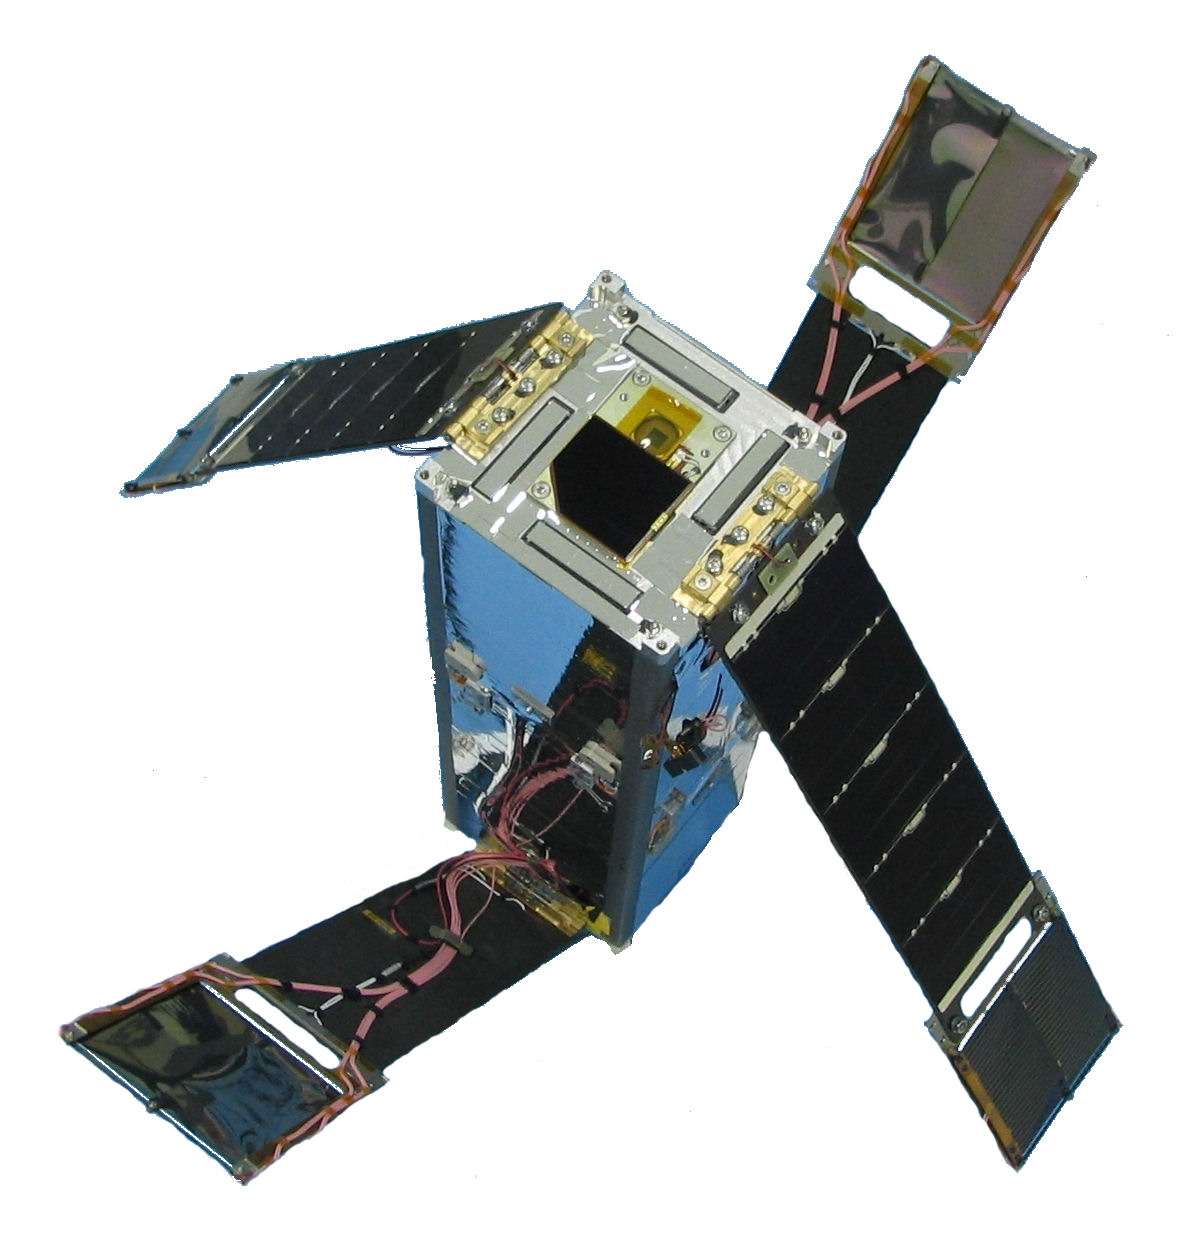
\includegraphics[width=8cm]{pics/Delfi-C3}
\end{center}
\hfill\parbox{5cm}{
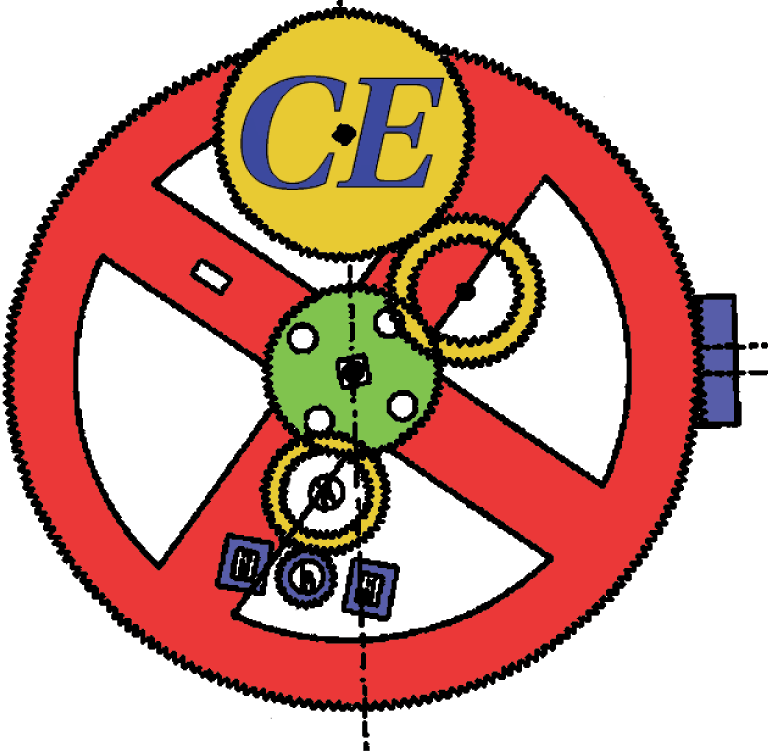
\includegraphics[width=3cm]{pics/CE_conv}}
\hspace*{2cm}\\



\vspace*{1.5cm}
\noindent

\includegraphics[width=\textwidth]{pics/TU_border_A4_L_front}
\end{textblock*}

\null\newpage


%%%%%%%%%%%%%%%%%%%%%%%%%%%%%%%%%%%%%%%%%%%%%%%%%%%%%%%%%%%%%%%%%%%%%%%%%%%%%%%
\hoffset=1.63cm
\oddsidemargin=0in
\evensidemargin=0in
\textwidth=5in

%%%%%%%%%%%%%%%%%%%%%%%%%%%%%%%%%%%%%%%%%%%%%%%%%%%%%%%%%%%%%%%%%%%%%%%%%%%%%%%
\parindent=1em

% EMPTY PAGE
\cleardoublepage

\pagestyle{plain}
\pagenumbering{roman}
\setcounter{page}{1}

% TITLE PAGE: page i (hidden)
\begin{titlepage}

  \begin{center}
  \null\vfill
    \begin{center}
    \LARGE{\reportTitle}
    \end{center}

    \vspace{3cm}

    \begin{large}
    Master's Thesis in \reportMSC
    \end{large}

    \vspace{1.5cm}

    \begin{normalsize}
    Computer Engineering Section\\
    Faculty of Electrical Engineering, Mathematics and Computer Science\\
    Delft University of Technology\\
    Mekelweg 4, 2628 CD Delft, The Netherlands
    \end{normalsize}

    \vspace{2.0cm}

    \begin{normalsize}
    \reportAuthor \\
    \reportUrlEmail
    \end{normalsize}

    \vspace{1.0cm}

    % <MM> DD, YYYY
    \reportDate             %TODO: Dit is de datum van uitgifte van final versie aan de afstudeer commissie

  \vfill
  \end{center}

\end{titlepage}


% GRADUATION DATA AND ABSTRACT: pages ii and iii (hidden)
%De aankondiging bevat de spreker, titel, plaats, datum en tijd, samenstelling van de afstudeercommissie en een korte samenvatting (maximaal 25 regels).
\thispagestyle{empty}

\noindent \textbf{Pranav Sailesh Mani}\\
\begin{tabular}{l}
\reportAuthor{} (\reportUrlEmail)\\
\end{tabular}\\
\noindent \textbf{Title}\\
\begin{tabular}{l}
\reportTitle\\
\end{tabular}\\
\noindent \textbf{MSc presentation}\\
\begin{tabular}{l}
% <MM> DD, YYYY (like \today)
30 November, 2017\\
\end{tabular}

\vspace{1.1cm}

\noindent \textbf{Graduation Committee}\\
\begin{tabular}{ll}
\graduationCommittee
\end{tabular}
\vspace{1.1cm}

\noindent \begin{tabular}{ll}
\textbf{Thesis Number - CE-MS-2017-14}
\end{tabular}

\begin{abstract} %de abstract bevat alleen een korte samenvatting van de inhoud van het onderzoek
\setcounter{page}{3}
\reportAbstract{ Cameras are used in various applications and one such common application has been space. Delfi Space is the CubeSat Development program of the Delft University of Technology and a subprogram of Defi-Space is Delfi-PQ which aims to develop PocketQubes which are an order of magnitude smaller than the CubeSat standards. One of the advanced payloads that would potentially be a part of the Delfi-PQ is an imager/camera. The imager needs to be as small as possible in order to fit into the Delfi-PQ satellites. The design of the camera has remained the same throughout the years and one of the reasons that increase the thickness of the camera is the presence of lenses. A way to reduce the size of the camera would be to remove the lens out of the equation. However, this introduces additional problems and trade-offs in the camera. These lenses can be replaced by masks/coded apertures. One of the additional steps in using coded-apertures is that additional computational steps need to be performed in order to reconstruct the image. The kind of computation that needs to be performed depends on the kind of masks that would be used. In this thesis, a separable mask is chosen and computer simulations on separable masks have been performed. Two image sensors that can be used in the picosatellite were chosen for implementation and the hardware/software is designed and developed. The experimental setup for determining the field of view of a lensless camera has been developed and tested. One of the trade-offs observed through the experiments is that the acceptance angle of a lensless imager had reduced by 38 percent and 31.8 percent in the horizontal and vertical directions compared to a conventional lens-based system. Based on the experimental results, the field of view of the camera has also been determined. A singular value decomposition based method has been developed and is used to align and calibrate the camera with the mask. The final step is estimating the system matrices of the lensless system. The system matrices enable the perfect reconstruction and a complete realization of a separable mask based lensless camera.  A scheme for estimating the system matrices of the lensless imager using Hadamard basis is proposed and confirmed using simulations and the strategy for experimental verification is proposed. As far as we know, this is the first study that focuses on designing and developing a lensless camera in the visible light domain for use in picosatellites. }
\end{abstract}

\clearpage

%\setcounter{page}{4}

% EMPTY PAGE: page iv
\cleardoublepage

% OPTIONAL QUOTATION: page v
%\pagestyle{empty}

\null\vfill

\begin{center}
\emph{``TODO QUOTE''} -- TODO QUOTED PERSON
\end{center}

\vspace{10cm}

\clearpage


% EMPTY PAGE: page vi
%\cleardoublepage

% PREFACE: page v
\chapter*{Preface}
\addcontentsline{toc}{chapter}{Preface}
This document contains the work that I have been doing for the past eight months. These months just flew by and I enjoyed working in this multi-disciplinary project. Firstly, I am thankful to the almighty for providing me the strength to overcome various challenges I faced over the past two years of my master program which has been highly demanding. I have a long list of people whom I would like to thank and without whose support this project could not have been completed.
I would like to first thank my parents for providing me the financial support for coming to the Netherlands and doing my master studies at TU Delft. Without their encouragement and support, I would not be where I am now. Next, I would like to thank my master program co-ordinator and my supervisor, Arjan van Genderen who accepted to supervise me in this multi-disciplinary project. I would like to thank Delfi Space Program Manager, Mr. Jasper Bouwmeester, who first introduced me to my second supervisor Hans Kuiper. Hans provided me the support and was instrumental in understanding the requirements for designing the imager. Next, I would like to thank the Paul Urbach who introduced me to the Optica Research Group which is where I did all the experiments. I am extremely thankful to Phd students, Yifeng Shao and Sander Kojninberg. Yifeng was also my daily supervisor and helped me with understanding the theoretical physics, simulation of imaging algorithms and also on how to work with optical instruments. He continuously encouraged me to overcome challenges I faced along the way. I could not have asked for a better supervisor. I would also like to thank Sander for many discussions that very highly insightful and helped me to cross hurdles that I faced. On the whole, the Optica Research Group was a very nice place to work with very sociable people. Lastly, I would like to thank my friends in Delft for their support and encouraging words in stressful times. 



\noindent
Delft, The Netherlands

\noindent
\today

% EMPTY PAGE: page vi
\cleardoublepage

% TABLE OF CONTENTS: starting at page vii
\tableofcontents

\cleardoublepage

\pagenumbering{arabic}
\setcounter{page}{1}

% INTRODUCTION: page 1
\chapter{Introduction and Problem Statement}
\label{chp:introduction}
The history of cameras go back to 13th century when Aristotle first noticed how light passing through a small hole in a darkened room produced an image of the sun on the wall. 
Throughout the centuries, the basic design of cameras have been continuously changing with  different versions of the 'camera obscura' with a single pinhole being developed by different civilisations. In a pinhole camera, light passes through the pinhole and forms an image on the sensor/image plane.
As the size of the pinhole increased, the quality of image formed on the plane decreased and as the pinhole size became smaller, lesser light was allowed which resulted in decreased field of view. With the development of science and due to the limitations of the pinhole, lenses were introduced to increase the size of the aperture, the sharpness of the image and the light throughput. As humanity progressed with the rapid pace in technology, we were able to capture images and store them on a film. With the digital explosion in early 1990s, the thin films were replaced by Charged Couple Devices(CCD). Then came the cameras based on Complementary Metal Oxide Semiconductors(CMOS). CCD and CMOS sensors reduced the size of cameras considerably and it was possible to develop low cost cameras in a large number. However, cameras have retained the lens throughout the years. Cameras are used for various applications and one such application is the space exploration domain. Delfi Space is the small satellite program of TU Delft that is mainly meant for education and technology demonstration in very small sized satellites. Delfi-PQ programme is a sub-programme of the Delfi Space programme that aims at developing extremely small but highly capable PocketQube satellites. PocketQubes are an order of magnitude smaller than the well known CubeSat standard which formed the basis of previous Delfi satellite projects. The dimensions of a PocketQube satellite would be 50mm * 50mm * 178mm and their volume would be approximately eight times smaller than CubeSats. 
One of the advanced payload that would be part of the Delfi-PQ would be an imager/camera that consumes extremely low power and would fit into the dimensions and power specified by the Delfi-PQ team.
 
In order to reduce the size of a camera, it would be necessary to remove the lens from the camera as the thinnest lens based mobile camera is 5mm thick. The primary focus of a lens would be to focus light from distant objects onto the CMOS sensor. Light from distant objects reach the sensor even without the lens except that the light is incoherent and the CMOS sensor would not be able to form the object properly without a lens. However, the lens could also be replaced by coded apertures. Coded Apertures have been used in the late 20th century to image X-Ray sources of light. Lensless coded aperture cameras can be as small as $100 \mu m$ thick. By using lensless cameras, we could potentially reduce the form-facto multiple times to suit the requirements of Delfi-PQ. However, the thesis would focus on the broader applications of lensless camera in satellites and would also make an attempt at addressing the power and computational requirements of the Delfi-PQ.

The thesis would be addressing the following research questions:
\begin{itemize}
\item Would it be possible to design a lensless camera to capture astronomical objects in the visible range of light spectrum?
\item What would be the minimum possible form-factor that would be achievable and the effects of different factors such as diffraction effects, mask-to-sensor distance and reconstruction algorithms?
\item If possible, how would the lensless camera compare with the conventional lens based cameras used currently?
\item Would it be possible to design a lensless camera that would fit the power and size constraints of the Delfi-PQ?
\end{itemize}
\vspace{1\baselineskip}

\noindent




% CHAPTERS ... For instance: History/Prior Work, Design/Implementation, Experiments
\chapter{Literature Survey and Trade-off Analysis}
\label{chp:LitSurvey}
In this chapter, a state-of-the art study will be presented that could assist in design of the lensless imager with specifications mentioned in the previous chapter.
\section{Camera Computational Pipeline}
In order to design a lensless imaging system, we must first look at the computational imaging pipeline of existing cameras. Since the lensless camera basically uses computation to reconstruct images, it is important to understand the computational pipeline of existing camera systems and make necessary modification in the design of the existing pipeline to suit the system. The computational imaging pipeline of existing camera systems is shown figure \ref{fig:CompPipeline}\cite{CompPipeline}.
\begin{figure}[htb]
% most GNUplot figures need to be rotated, width should be the same throughout the complete document, and no extension is needed
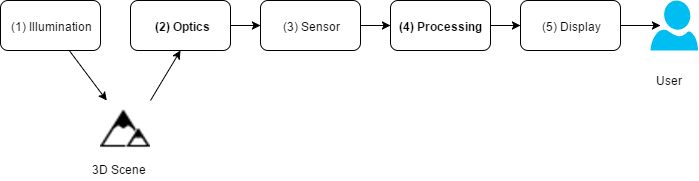
\includegraphics[width=\textwidth]{pics/CompPipeline}
\caption{Computational Pipeline of Existing cameras}
\label{fig:CompPipeline}
\end{figure}
As shown in figure \ref{fig:CompPipeline}, there are five main components that can be controlled computationally in existing systems. Illumination of the scene can be controlled to produce an enhanced picture. Optics could be controlled to limit the amount of light entering the scene and thereby controlling the image produced on the sensor. The sensor can also computationally modify the date it receives to de-noise, adjust the blackness/white in an image. Post-processing can also be done on the image produced by the sensor to improve the image produced by the sensor. Finally, a display can also be modified computationally to produce certain effects on the user. And of course, the user can control any of these components to produce the effect he desires. But in the case of the lensless imaging system, we would be modifying the optics and the processing components of the pipeline to reduce the size of the camera.The components to be modified are are darkened in figure \ref{fig:CompPipeline}. 

\section{Satellite Imaging Architectures}
Since the camera is going to be capturing pictures of the earth, it would be required to study the existing imaging architectures currently being used in satellites and how the design of the lensless camera would fit into the existing imaging architectures. We will first look into the terminology commonly used in space instrumentation. As the imager is carried along the orbit of the earth, it images a strip on the surface of the earth. The width of the strip is called the 'swath'. The direction along which the satellite moves or images is called the 'along-track' direction and the direction perpendicular to it is called the cross-track direction\cite{ImagingGeo}. Figure \ref{fig:ImagingGeo} describes these terminology and some other terms as well.  
\begin{figure}[ht]
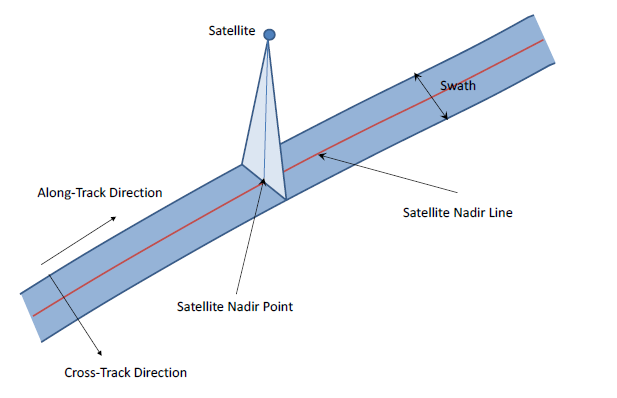
\includegraphics[width=\textwidth]{pics/imaginggeo}
\caption{Various Imaging Terms\cite{ImagingGeo}}
\label{fig:ImagingGeo}
\end{figure}
Three major types of scanning architectures are employed in space instruments, namely:
\begin{itemize}
\item Whiskbroom Line Scanner: In this type of scanning architecture, a detector element detects it's instantaneous field of view which is projected onto a pixel element. In this scanning type the surface of the earth is scanned in lines. A scanning mirror would project a very small area of the earth onto the single pixel element. The scanning mirror would then rotate to project the next element of the line onto the next pixel. Depending on the motion of the satellite, the next line of the detector is scanned and projected on to the next line on the surface of the earth. An advantage of this type of detector is that it would be possible to obtain a very large field of view. However, it also comes with disadvantage that a very high sampling frequency is required to get decent resolutions. Typically, an earth observation satellite would move at 6.5 km per second. In order to get a resolution of 100 meters per pixel, it would be required to sample atleast 65 lines per second. For a swath of 1000 pixels it would be required to sample at 65000 elements per second. Apart from this, there is very limited time for each detector element which would result in low spatial resolution\cite{SpInst}. Another main disadvantage is that mechanical components would be required to project different parts of the surface of the earth on to the detector element. This type of scanner is also called as along-track scanner. Mathematically, the measurement of the detector element $(X,Y)$ can be described using 
$$
(X,Y) = f(t_x, t_y)
$$
where $t_x$ and $t_y$ is the time at which the image is captured in the corresponding location
%\begin{figure}[ht]
%\begin{subfigure}
%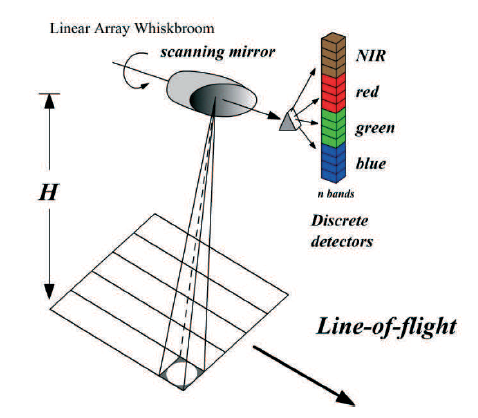
\includegraphics[width=0.5\textwidth]{pics/WhiskBroom}
%\caption{Whiskbroom Scaning Architecture}
%\label{fig:WhiskBroom}
%\end{subfigure}
%\begin{subfigure}
%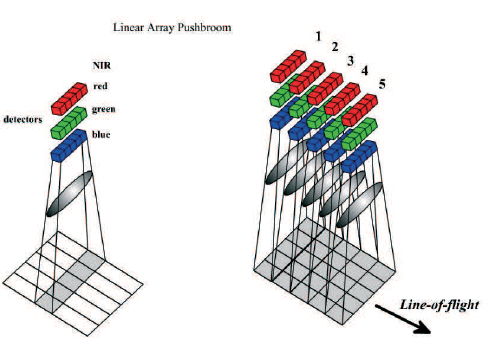
\includegraphics[width=0.5\textwidth]{pics/PushBroom}
%\caption{Pushbroom Scaning Architecture}
%\label{fig:PushBroom}
%\end{subfigure}
%\end{figure}
\begin{figure}[ht]
\centering
\begin{subfigure}{0.75\textwidth}
  \centering
  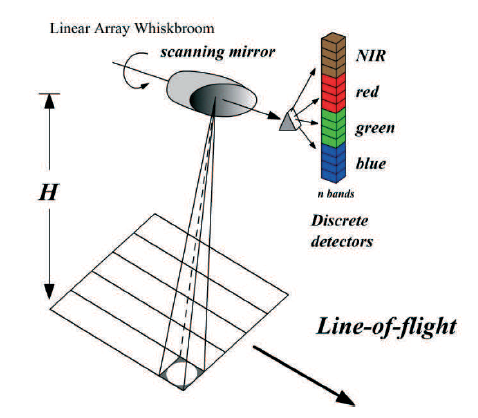
\includegraphics[width=.5\linewidth]{pics/WhiskBroom}
  \caption{WhiskBroom Scanning}
  \label{fig:Whiskbroom}
\end{subfigure}
\begin{subfigure}{0.75\textwidth}
  \centering
  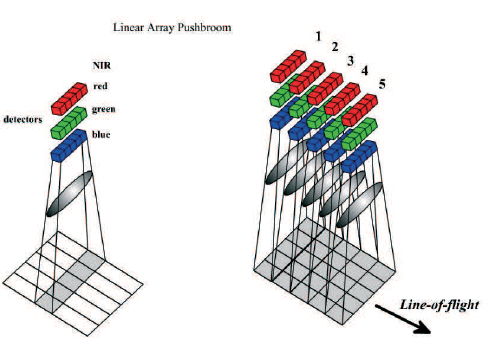
\includegraphics[width=.65\linewidth]{pics/PushBroom}
  \caption{Pushbroom Scanning}
  \label{fig:Pushbroom}
\end{subfigure}
\caption{Push Broom and Whisk Broom Scanning}
\label{fig:test}
\end{figure}

\item Pushbroom Line Scanner : In this type of architecture, the orbital motion of the sensor is used to image the swath instead of using a mirror as in the case of whiskbroom scanner. The field of view in the cross-track direction is imaged by the corresponding line detector array. Successive lines are imaged and sampled by the multiplexer as the sensor moves across the surface. The time between sampling two successive lines can be the time it takes for the satellite to move that distance. The most commonly used detector for a pushbroom scanner is Charge Coupled Devices(CCD). One of the main advantages of this type of scanner is that it requires no moving parts. Due to this, it is possible to obtain very high scanning rates(< $1 \mu$ second). This also leads to lower noise in the received signal\cite{SpInst}. The disadvantage is that large number of detectors are required to image a large piece of area. In addition to this, it requires an optical arrangement that could obtain a wide field of view. Mathematically, the measurement of the detector element $(X,Y)$ can be described using 
$$
(X,Y) = f(x), f(t_y)
$$
where $f(x)$ represents the sensor output and $f(t_y)$ represents the time at which the subsequent rows are imaged.  
\item Staring Array : Staring arrays use 2-d CCD/CMOS detectors to capture an entire area on the surface of the earth. These are also called as framing cameras. This provides speed-up and step-and-stare mechanism is employed wherein observations are made intermittently after a certain number of steps in the cross-track direction. The advantage is that moderate field of view optics is only required in this case\cite{SpInst}. Mathematically, the measurement of the detector element $(X,Y)$ can be described using 
$$
(X,Y) = f(x), f(y)
$$
where $f(x)$ and $f(y)$ represents the sensor output.
\end{itemize}
\section{Trade-off Analysis}
\label{sec:tradeOff}
\subsection{Camera Sensor}
The camera sensor is the core of the Delfi-PQ Imager. The performance of a camera is mainly limited by the image sensor that it uses\cite{cmos}. The camera sensor can be off two types namely, CCD(charge coupled device) or CMOS(Complimentary Metal Oxide Semiconductor). Both the types of CMOS sensors have their own advantages and disadvantages. To understand the challenges that each type of sensor poses, we must understand how the sensors are designed.

The following factors have been chosen to  make a trade-off between the different CMOS sensors:
\begin{enumerate}
\item Resolution : When rating a camera, the first thing that comes to the mind is the resolution of the camera. The resolution of a camera is directly dependent on the number of pixels in the image sensor of the camera. 
\item Power Consumption : In the design of the PQ-Camera, the most important factor is the power consumption of the entire imager. The majority of the power consumption by the imager is dependent on the power consumption of the CMOS sensor. 
\item Availability : Even though there are innumerable number of CMOS sensors in the world, availability of CMOS sensors is quite low when it comes to small-scale. Many CMOS manufacturers require large scale orders.
\item Quantum Efficiency(QE) : Quantum Efficiency is the measure of efficiency of the camera sensor to convert incoming photons into electrons. The ratio of electrons generated during the digitization process to photons is called quantum efficiency.
\item Pixel Size : Pixel size is the size of each pixel unit in the CMOS camera. It is also an important factor considering that the signal produced by the CMOS sensor depends on the pixel size as well.
$$
Signal = Light Density * (Pixel Size)^2 * QE
$$
\item Electronic Interface : The electronic interface that can be used to retreive data from the CMOS sensor also plays an important role. Since the project uses a low-power microcontroller that has limited communication capabilities, it would be wise to chose an interface that is supported by the microcontroller. Recently available chips use LVDS/MIPI interface to send data. These interfaces are not supported by the microcontroller that is being used as an on-board computer. The on-board computer uses an I2C based interface and that the electronic interface would be an important factor as it would reduce the complexity of the system and also reduce the power consumption by removing the addidional circuitry necessary for interfacing with the onboard computer.

\item Dynamic Range : Dynamic Range and SNR are used interchangeably in CMOS sensors. The only difference is that dynamic range considers only the temporal dark noise while SNR includes the root mean square of the shot noise as well.  

\item Shutter Type : Camera sensors use different types of shutters namely, global shutter and rolling shutter. Global shutter reduces the distortions due to fast moving artefacts while increasing the dark current. Rolling shutter has more distortions in the case of imaging moving artefacts, but also has lesser dark noise compared to global shutter. 

\item Voltage Level : Voltage level also has to be taken into account while choosing the sensor because if the CMOS sensor needs a voltage level higher than that of the main satellite bus voltage, then additional circuitry has to be introduced to step up the voltage level which in turn increases the overall system power.  

\item Operating Temperature : Operating temperature is an important factor to take into account when choosing an imaging sensor. Since the camera is going to operate in space, it is better if the CMOS sensor has a higher operating range of temperature. 

\item Overall Size and Weight : As the imager has to fit within specific dimensions, the overall size and weight of the CMOS sensor also needs to be taken into account.

\item Frame Rate: Even though, it is not required to have a camera sensor that is capable of high frame rates, it is an added advantage and higher frame rate camera could help in imaging larger areas of the earth if required. 
\item Price: While there are no specific cost constraints in the project, price has also been taken into account.
\end{enumerate}

In \cite{surveyCamMod}, a survey of camera modules for a CubeSat space Mission has already been carried. However, we also consider image sensors(not same as camera modules) as we are fundamentally changing the design of a camera. 

The following candidates have been chosen for analysis. These candidates are chosen based on \cite{surveyCamMod} and also on the latest CMOS sensors available on the market. 
\begin{enumerate}[label=(\alph*)]
\item IDS UI- 1646LE USB 1.3MP
\item C3188A
\item PC67XC-2 CCD
\item MicroCam TTL
\item PB-MV40
\item Omnivision OV7670
\item Sony ICX285AL
\item Omnivision OV5642
\item Omnivision OV2740
\item MCM20027
\end{enumerate}

\begin{table}[ht]
\caption{Comparison of Different Image Sensor Candidates}
\label{tbl:TradeoffCMOS}
\begin{tabular}{|c|c|c|c|c|c|c|c|c|c|c|}
\hline
\diaghead{\theadfont Diag ColumnmnHead II}%
{Factors}{Candidates}&
\thead{(a)}&\thead{(b)}&\thead{(c)}&\thead{(d)}&\thead{(e)}&\thead{(f)}&\thead{(g)}&\thead{(h)}&\thead{(i)}&\thead{(j)}\\
\hline
\textbf{Optical Parameters} & & & & & & & & & &\\
\hline
Resolution & ++ & + & + & - & ++ & + & ++ & ++ & ++ & ++ \\
\hline
Pixel Size & + & ++ & X & ++ & ++ & + & ++ & + & + & ++ \\
\hline
Shutter type & - & - & X & - & - & + & + & + & + & - \\
\hline
Frame Rate & + & + & + & + & +++ & + & + & + & + & + \\
\hline
\textbf{\makecell{Electrical and \\other parameters}} & & & & & & & & & & \\
\hline
Power Consumption & - - & - -  & - - - & ++ & - & ++ & - & - - - & - -& - - \\
\hline
Availability & - & + & - - - & - - -& - - - & ++ & - - & ++& - -& - - -\\
\hline
Electronic Interface & + & + & - - - & ++ & - - & ++ & - - & ++ & - & +\\
\hline
DR and SNR & X & + & X & ++ & + & ++ & + & ++& + & +\\
\hline
Voltage & + & + & - - - & ++ & + & ++ & + & ++ & - & +\\
\hline
Operating Temperature & + & + & + & + & + & + & + & + & + & +\\
\hline
Overall Size and Weight & + & + & + & + & + & + & + & + & + & + \\
\hline
Price & - & + & X & X & - - - & ++ & X & + & X & X\\
\hline
\textbf{Points} & 2 & 8 & -8 & 8 & 0 & 18 & 5 & 13 & 2 & 4\\
\hline
\end{tabular}
\end{table}

\subsection{Compression Algorithms}
Data Compression plays a very important role when it comes to space missions. It is a very important aspect in the system design of a lensless camera for space application as the image that needs to be sent down to earth needs to be compressed as much as possible. Various surveys\cite{Compression2}\cite{Compression3}\cite{Compression4} have been conducted previously in-terms of which compression algorithm would best preserve the data and provide maximum compression at the same-time. Compression algorithms can be divided into two types namely lossy and lossless. Lossless compression algorithms are algorithms in which we can reconstruct the original image without any loss in data. Typical examples of lossless algorithms include Portable Network Graphics Format(PNG), Bitmap Format(BMP), TIFF(Tagged Image File Format). Lossy compression algorithms are compression algorithms in which we cannot completely reconstruct the original image. However, lossy compression factors offer a very high compression ratio compared to loss-less algorithms. Lossy Compression algorithms include DCT(Discreet Cosine Transform), JPEG(Joint Photographic Experts Group), SPIHT(Set Partitioning in Hierarchical Trees)\cite{Compression3}. A survey conducted for European Student Moon Orbiter Mission\cite{Compression3} has reviewed various possible compression algorithms that could be used for lunar imaging. The compression algorithms were evaluated on the basis of Mean Square Error(MSE), Peak Signal to Noise Ratio(PSNR), Normalized Cross-Correlation(NK), Averaged Difference(AD), Structural Content(SC), Maximal Difference and Normalized Absolute Error(NAED). The reviewed compression formats were BMP, CGM, GIF, JPEG, PNG, TIFF, WebP. Loss-less compression generally does not offer a compression ratio of more than 2 due to the entropy present in real-life artefacts. Since space missions offer a limited communication link-speed, the compression ratio needs to be more than 2. This cannot be offered by lossless compression and hence we need to go for lossy compression formats. It can be seen from table \cite{tbl:TradeoffCompression} that JPEG and SPIHT perform better compared to DCT. It can be seen that JPEG offers better performance in-terms of Mean Squared Error. However, SPIHT offers a higher compression ratio. 

\begin{table}[ht]
\caption{Ranking of Different Compression Algorithms}
\label{tbl:TradeoffCompression}
\begin{tabular}{|c|c|c|c|c|c|}
\hline
\diaghead{\theadfont Diag ColumnmnHead II}%
{Method}{Factors}&\thead{MSE}&\thead{PSNR}&\thead{AD} &Compression Ratio& Implementation Needed\\
\hline
JPEG & 1 & 1 & 1&2&No\\
\hline
DCT(With Zip) & 2& 2& 1& 3&No\\
\hline
SPIHT & 3& 1& 1&1&Yes\\
\hline
\end{tabular}
\end{table}
JPEG algorithm is chosen for implementation since it offers equivalent performance to SPIHT and JPEG compression engine is present in most of the commercially available CMOS/CCD sensors.

The JPEG compression algorithm is comprised of the following steps.
\begin{itemize}
\item
\end{itemize}


\begin{figure}[]
\centering
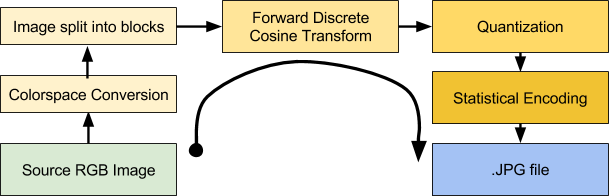
\includegraphics[scale=0.50]{pics/jpegcompression.png}
\caption{Steps involved in JPEG Compression\cite{Jpeg}}
\label{fig:Rec_Acc}
\end{figure}

\begin{figure}[]
\centering
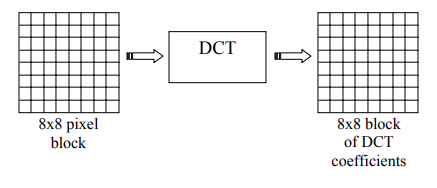
\includegraphics[scale=1]{pics/dct.PNG}
\caption{DCT involved in JPEG\cite{dct}}
\label{fig:Rec_Acc}
\end{figure}
\subsection{Masks and Reconstruction Algorithms}
The main aim of designing a lensless camera is that it would help reduce the size of the camera considerably. In a lensed camera, light emanating from multiple-points in the object would intersect to form the image of the object. This is illustrated in Figure \ref{fig:lens_image}. the focal length of the lens-involed primarily determines the thickness of the camera(See Figure \ref{fig:focal_length}). In a lensless, imaging system the lens is replaced by means of a mask(series of pinholes arranged in a periodic manner). This is illustrated in Figure \ref{fig:lensvslensless}.
\begin{figure}[ht]
\centering
\begin{subfigure}{0.75\textwidth}
  \centering
  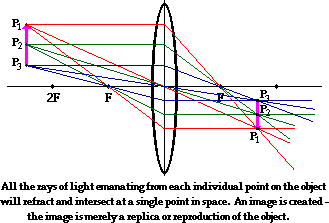
\includegraphics[width=.5\linewidth]{pics/lensed_image_formation}
  \caption{Image Formation in a lens-based camera\cite{lens1}}
  \label{fig:lens_image}
\end{subfigure}
\begin{subfigure}{0.75\textwidth}
  \centering
  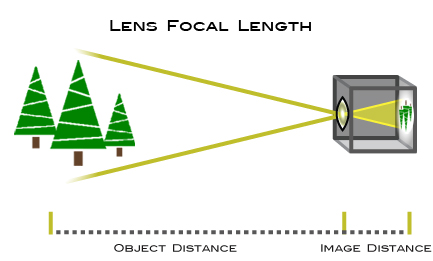
\includegraphics[width=.65\linewidth]{pics/focal_length}
  \caption{Relation between focal length and thickness\cite{lens2}}
  \label{fig:focal_length}
\end{subfigure}
\caption{Lens-based Camera}
\label{fig:lens_based}
\end{figure}

The simplest lensless imaging system is the pinhole camera. However, since the quality of the image depends on the size of the pinhole, that restricts the amount of light that can enter the imaging system. Lenses were introduced to focus the light from distant objects onto a film or a sensor. In the absence of a lens, the sensor would record the average intensity of the light entering it. This can also bee seen in the experiments which are described in the upcoming chapters. 
\begin{figure}[ht]
\centering
\begin{subfigure}{\textwidth}
  \centering
  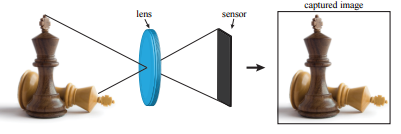
\includegraphics[width=0.75\linewidth]{pics/lensless_1}
  \caption{Conventional Lensed Imaging}
  \label{fig:lensed_imaging}
\end{subfigure}
\begin{subfigure}{\textwidth}
  \centering
  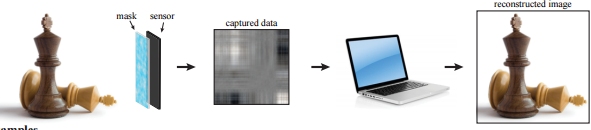
\includegraphics[width=0.75\linewidth]{pics/lensless_2}
  \caption{Lensless Imaging}
  \label{fig:lensless_imaging}
\end{subfigure}
\caption{Difference between lensed and lensless imaging methods\cite{VBoomi}}
\label{fig:lensvslensless}
\end{figure}

Before lenses, 



Coded aperture cameras extend the pinhole camera concept replacing the single aperture with a mask containing multiple apertures. The first developed coded aperture cameras were used in imaging X-Ray sources due to the difficulty involved in focussing light from X-Ray sources\cite{Cannon1}. Since a single pinhole limits the amount of light imaged by the sensing element, it was replaced by many holes, called the aperture so that overlapping images are formed on the film. The recorded image will have no similarity with the source and an digital processing is required to reconstruct the source image or the object. The recorded image is mathematically modelled as a  collection of overlapping shadows as described by the following equation\cite{VBoomi}\cite{Cannon1} 
\begin{equation}
y = \phi * x + e
\end{equation}

where $y$ represents the image formed on the sensor, $\phi$ represents the mask pattern, $x$ represents the irradiance vector or the object and $e$ represents the noise. The $*$ operator represents the convolution operation between the mask an the object. The coded aperture increases the flux that falls on the detector and this leads to an increase in the SNR. The SNR can be as large $\sqrt{N}$, where N represents the number of holes in the aperture\cite{Cannon1}. The increased SNR comes at the cost of computational decoding for the image. 
\chapter{Simulation of Reconstruction Algorithm}
This chapter will describe how the system can be mathematically modelled and how the mask for the lensless imager was designed. As mentioned in the previous chapter the system can be modelled as 
\begin{equation}
\label{eq:conv2}
I = M * x + e ;
\end{equation}
where $x$ refers to the object scene, $M$ represents the mask function and $I$ represents the image formed on the sensor. Ignoring the noise and converting the equation to fourier domain, the equation \ref{eq:conv2} can be re-written as
\begin{equation}
\label{eq:conv3}
F(y) = F(\phi)F(x)
\end{equation}
\begin{equation}
\label{eq:conv3}
F(x) = \frac{F(y)}{F(\phi)}
\end{equation}
\begin{equation}
\label{eq:conv4}
x = F^{-1}(\frac{F(y)}{F(\phi)})
\end{equation}
Equation \ref{eq:conv4} is the simplest possible computational inversion of the scene from the sensor. This method has also been used in \cite{Toeplitz}. As mentioned in the previous chapter, there are two types of masks that can be used for the purpose of encoding the scene onto the mask, namely separable and non-separable mask. MATLAB has been used for the purpose of simulating the algorithms. In this chapter, we would simulate two types of mask patterns, namely separable and non-separable mask patterns. A separable mask pattern is one in which the mask matrix $\phi$ can be expressed in-terms of two sub- matrices:
\begin{equation}
M = M_A * M_B
\end{equation}
Both $M_A$ and $M_B$ are doubly-toeplitz mask. The mathematical model is also changed as described by the equation \ref{eq:separable}. A non-separable mask is one which does not follow this property.

\section{Simulation of a non-separable mask}
The non-separable mask simulation was carried out as shown in Figure \ref{fig:non_sep_sim}. Due to the inherent ill-posed mathematics involved in imaging extended scenes, a regularization term is added to the inversion process and we get equation \ref{eq:conv5}. This kind of regularization is called Tikhonov regularization. It regularizes the inversion, removes the zero valued elements in the mask fourier transform and controls the effects of noise\cite{Toeplitz}. The same regularization is also used in previous studies\cite{Toeplitz}. The value of $k$ was optimally tuned to get the best possible reconstruction(See equation \ref{eq:conv5}).

\begin{equation}
\label{eq:conv5}
x = F^{-1}(\frac{F(y)}{F(\phi)+k})
\end{equation}
\begin{figure}[ht]
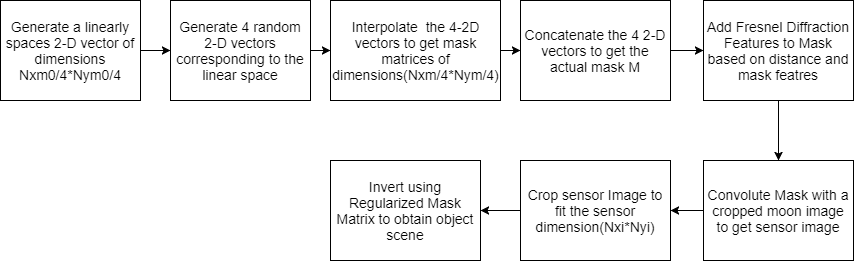
\includegraphics[width=\linewidth]{pics/non_sep_sim_flow}
\caption{Simulation-Flow non-separable mask}
\label{fig:non_sep_sim}
\end{figure}

In order to start with the mathematical modeling process and to imitate the sensor data and reconstruction, a reference image is needed. For that, it was decided to use the full moon image captured by the Apollo 11 space craft\cite{MoonImage}. Since the satellite is going to be pointing towards astronomical objects like the earth and the moon, it was decided to crop out a portion of the full moon image(See Figure \ref{fig:moon_image}). The simulation is done under the assumption that the camera is enclosed in a box-like structure and light from a specific region of the earth/moon would reach it and the sensor size is finite. The image was converted to gray and scaled down from 0 to 1 and is displayed in the \texttt{bone} colormap format available in MATLAB as the colormap would display the minute variations in the reconstructed image. This is illustrated in Figure \ref{fig:moon_image}. The simulation is performed and analyzed with and without diffraction . The mask used for simulation is shown in Figure \ref{fig:non_sep_sim}.
\begin{figure}[ht]
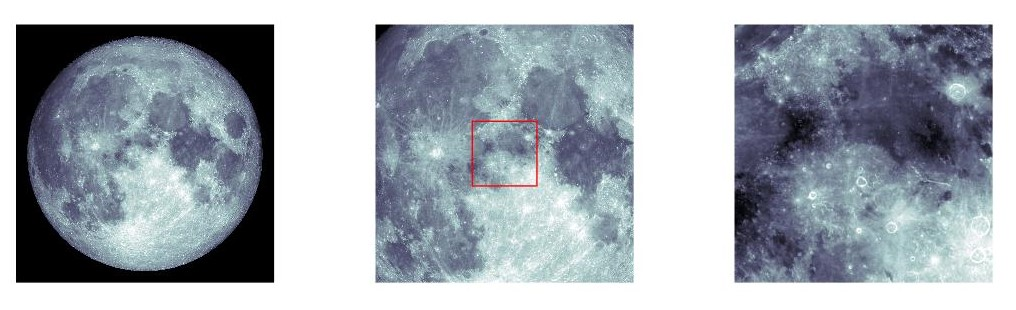
\includegraphics[scale = 0.50]{pics/MoonImagePortion}
\caption{The first image is the original image of the moon as taken by Apollo 11 spacecraft. The second image indicates the cropped region and the third image indicates the region that is used for the simulation.}
\label{fig:moon_image}
\end{figure}
The simulation parameters are shown in Table \ref{tbl:sim_parameters}. The reconstruction error is given by the equation \ref{eq:psnr}. $O_{guess}$ indicates the reconstruction and $O$ represents the original object. Fresnel diffraction features are added to the mask since the distance between the mask and the sensor lies in the Fresnel diffraction region and the Fresnel number for the mask is less than  1. The Fresnel diffraction modeling is described in the appendix section of the report.Diffraction causes the mask to become non-binary.
\begin{equation}
PSNR = 20log(\frac{N*max(O)}{MSE})
\label{eq:psnr}
\end{equation}
where 
\begin{equation}
MSE = \frac{1}{mn}\sum_{i=1}^{i=N}\sum_{j=1}^{j=N}[O(i,j) - O_{guess}(i,j)]^2
\end{equation}

\begin{table}
\caption{Simulation Parameters}
\begin{center}
\begin{tabular}{ |c|c| }
\hline
Pixel Size & 2.2$\mu m$ * 2.2$\mu m$\\
\hline
Sensor Size & 512 * 512 pixels\\
\hline     
Mask Size & 1024 * 1024 pixels\\
\hline 
Mask Sensor Distance & 5 millimeters \\
\hline 
\texttt{Nxm0, Nym0} & 256, 256\\
\hline
\end{tabular}
\label{tbl:sim_parameters}
\end{center}
\end{table}

\begin{figure}[ht]
\centering

\includegraphics[scale = 0.250]{pics/non_separable_mask}
\caption{Non-separable mask used for simulation}
\label{fig:non_sep_sim}
\end{figure}

\begin{figure}[ht]
\centering
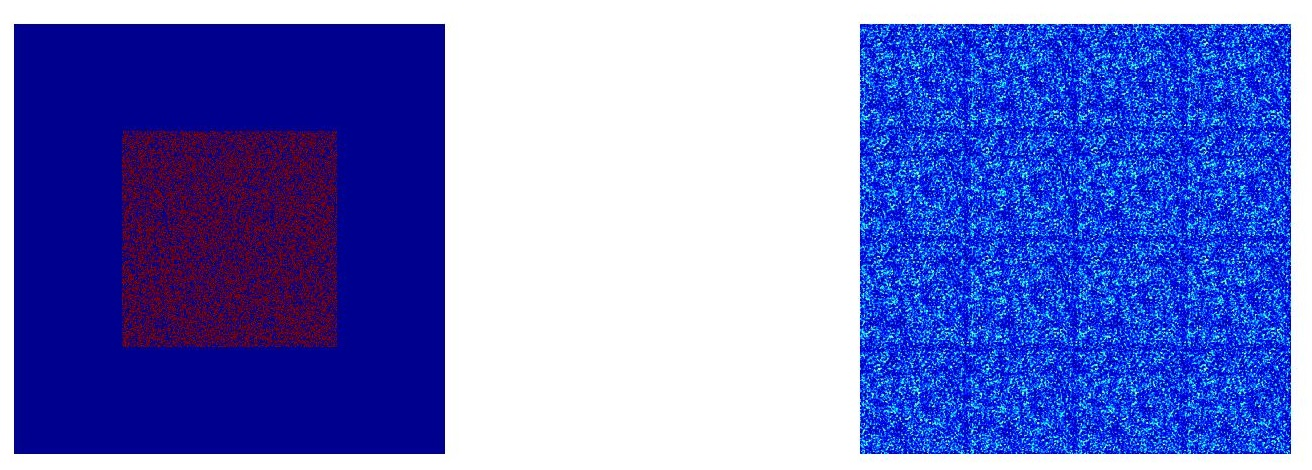
\includegraphics[width = \textwidth]{pics/non_sep_diffracted_mask}
\caption{The mask on the left indicates undiffracted mask and the mask on the right indicates the diffracted non-separable mask}
\label{fig:non_sep_sim_diff}
\end{figure}

\begin{figure}[ht]
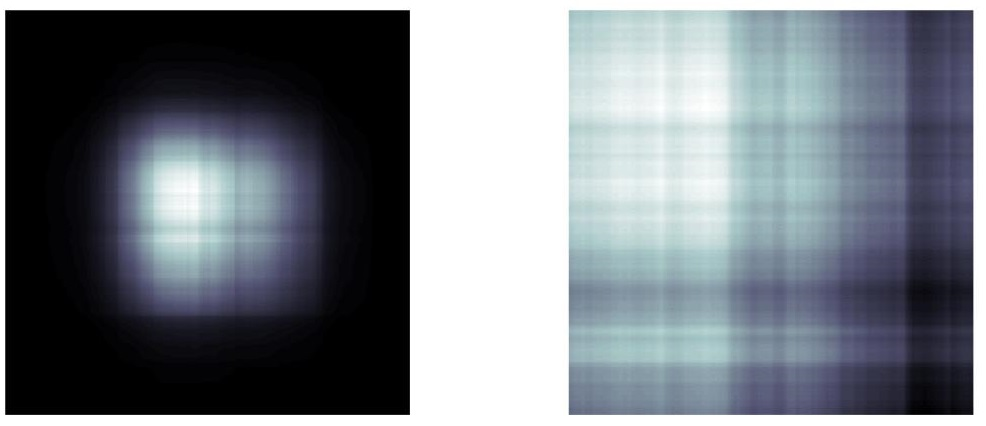
\includegraphics[scale = 0.50]{pics/sensorCropped}
\caption{The first image indicates the sensor image if the sensor plane was infinite. The second image indicates the cropped sensor image that would be formed on an actual finite sensor size(cropped).}
\label{fig:moon_image}
\end{figure}
The reconstructions obtained using equation \ref{eq:conv5} is shown in Figure \ref{fig:rec_non_sep}. It can be seen from the figure that we have successful reconstructions using equation \ref{eq:conv5}. The value of $k $ was set to 0.01. This value was found out by testing the reconstruction for different possible values and the value with the best possible reconstruction was chosen.
However, when the diffracted mask is modeled for the sensor image, the reconstruction fails. This is the reason why we need to go for the separable mask as this mask is not resistant to diffraction effects. 
  \begin{figure}[ht]
    \centering
    \begin{subfigure}{0.5\textwidth}
    \centering
        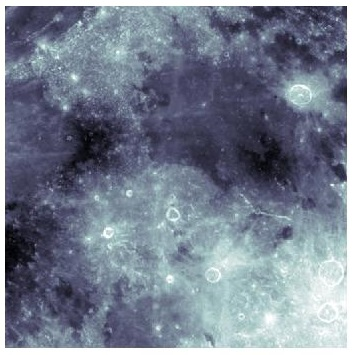
\includegraphics[scale = 0.5]{pics/rec_non_sep}
    
    \end{subfigure}%
    \begin{subfigure}{0.5\textwidth}
    \centering
        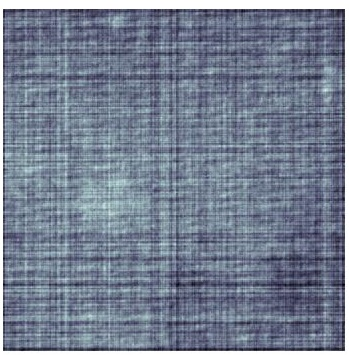
\includegraphics[scale= 0.5]{pics/rec_non_sep_diff}
    \end{subfigure}
    \caption{the figure shows the reconstruction with and without fresnel diffraction effects for a non-separable mask using equation \ref{eq:conv5}. We are able to obtain PSNR = 57.85 without diffraction effects. However, the reconstruction with the mask fails when diffraction effects are incorporated into the mask. }
    \label{fig:rec_non_sep}
    \end{figure}
    
    
\section{Simulation of a separable mask}
As we saw in the previous section, a non-separable mask cannot be used for our application in the visible light region as the visible light spectrum contains significant diffraction effects. We can improve the solution since a separable mask follows the equation \ref{eq:separable}. The same improved solution has been used in \cite{Toeplitz}. We can express \ref{eq:separable} as shown in equation \ref{eq:sep_sq}.
\begin{equation}
M_{A}^TIsM_{B} = (M_{A}^TM_{A})O(M_{B}^TM_B)^T 
\label{eq:sep_sq}
\end{equation} 
We multiply the left and right system matrices to obtain square symmetric matrices. The problem is that they are not invertible, due to the presence of zero eigenvalues. So, the parameters $\alpha_A$ and $\alpha_B$ to remove the zero eigenvalues and make them invertible. The final solution will be given by the equation \ref{eq:sep_final}.
\begin{equation}
O_{Guess} = (M_{A}^TM_A + \alpha_{A}^21_{R_{O}})^{-1}M_{A}^TIM_{B}(M_{B}^TM_B + \alpha_{B}^21_{C_{O}})^{-1}
\label{eq:sep_final}
\end{equation}
One more advantage of using the separable mask is the reduced amount of computation needed compared to the non-separable mask. The number of computations for a non-separable mask will be given by the equation \ref{eq:non_sep_comp}. For a megapixel image, this would translate to $10^{18}$.
\begin{equation}
N_{operations} \propto (r_O*c_O)^3
\label{eq:non_sep_comp}
\end{equation}

\begin{table}[ht]
\caption{Table indicating the rows and columns used for simulation}
\label{tbl:comp_sep}
\begin{center}
\begin{tabular}{ |c|c|c| }
\hline
Matrix & Rows & Columns \\
\hline
Mask Size & $r_M$ & $c_M$\\
\hline
Image on Sensor & $r_I$ & $c_I$\\
\hline
Object Area contributing &  $r_O = r_M + r_I - 1$ & $c_O = c_M + c_I - 1$\\
\hline
Left Toeplitz Mask & $r_{I}$ & $r_{O}$\\
\hline
Right Toeplitz Mask & $c_{I}$ & $c_{O}$\\
\hline
\end{tabular}
\end{center}
\end{table}


For a separable mask, however, the number of computation is drastically reduced because the size of the left and right system matrices is reduced to $(R_I*R_O)$ and $(C_I*C_O)$ from multiplying the entire object matrix of size $r_O*c_O$. This would come to around $2*10^9$ operations.This can also be observed in the simulation and it takes an extremely long amount of time to complete a non-separable matrix. The size of different matrices used in the simulation is shown in Table \ref{tbl:comp_sep}.

\begin{equation}
N_{operations} \propto [(r_I*r_O)^3 + (c_I*c_O)^3] 
\label{eq:sep_comp}
\end{equation}

The separable mask simulation was carried out as shown in Figure \ref{fig:sep_sim}. It is possible to generate different types of Toeplitz mask by simply changing the simulation variable \texttt{Nxm0}. These masks follow the same property and offer the same amount of reconstruction in the simulation. By changing \texttt{Nxm0}, the base vector that is used for interpolating to the bigger mask changes. This lead to different masks being generated. The shape of the mask is simpler when we use a smaller \texttt{Nxm0} as a very small vector is used for interpolation to get a bigger mask. The transmittance of the masks varies between 20 to 25 percent. The different masks obtained by changing \texttt{Nxm0} is shown in Figure \ref{fig:sep_mask_multi}. By changing the \texttt{Nxm0}, we can basically change the feature size of the mask. A lower \texttt{Nxm0} generates a mask where the subsequent binary value comes at a greater distance than the one with a larger \texttt{Nxm0}. It can be seen from figure \ref{fig:sep_sim} that there as an additional step involved in the simulation process of separable masks which is the rank-1 estimation of diffracted matrices. In this step, we perform Singular Value Decomposition(SVD) on the diffracted matrices to obtain $M_x$ and $M_y$. Now let us see what is singular value decomposition. Singular value decomposition is a mathematical tool that would enable us to express any matrix of the form $M_{ m \times n}$ in the form given by equation \ref{eq:svd_1}\cite{svd}. 

\begin{equation}
\label{eq:svd_1}
M_{m \times n} = U_{m \times r}S_{r\times r}(V_{n \times r})^T
\end{equation}
where $r$ represents the rank of the matrix $M$ , $m$ and $n$ denote the size of the matrix respectively. We can estimate the rank-1 estimation of a matrix by taking the first row and column of $U$ and $V$ and multiplying them as shown in equation \label{eq:svd_2}.

\begin{equation}
\label{eq:svd_2}
M_{1} = U_{1}S_1(V_{1})^T
\end{equation}
One of the main advantages of using a doubly Toeplitz mask is that it is decomposable into a single rank matrix with and without the effects of diffraction. The other rank-components are negligible even in the presence of diffraction. This is an important property that must be kept in mind which will be used for various experimental purposes.  In the simulation, we use SVD on the diffracted mask, take the rank-1 estimate of the mask. The $U_1$ and $V_1$ will represent the left and right system matrix of the refracted mask. The obtained single dimensional $U_1$ and $V_1$ of the doubly Toeplitz mask will be converted into Toeplitz matrices and inverted using equation \ref{eq:sep_final}. The decomposition of the diffracted and non-diffracted separable mask into a 1-rank matrix(with other components negligible) was also verified in the simulations.
The difference between diffracted and non-diffracted separable mask is shown in Figure \ref{fig:diff_separable}.
\begin{figure}[ht]
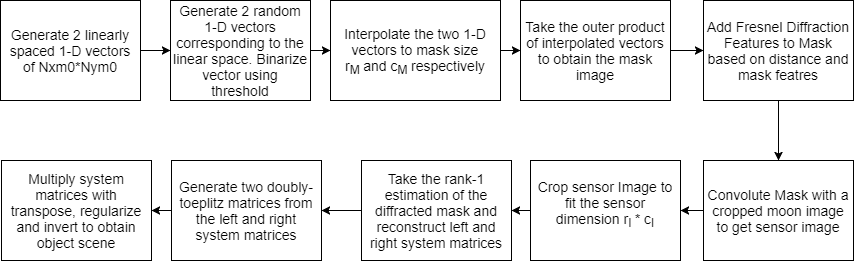
\includegraphics[width=\linewidth]{pics/sep_mask_sim_flow}
\caption{Simulation-Flow separable mask}
\label{fig:sep_sim}
\end{figure}
  \begin{figure}[ht]
    \centering
    \begin{subfigure}{0.5\textwidth}
    \centering
        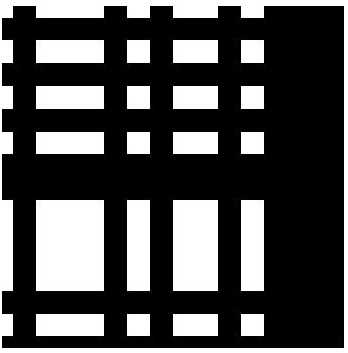
\includegraphics[width=0.5\linewidth]{pics/mask_16}
        \caption{\texttt{Nxm0} = 16}
        \label{fig:mask-16}
    \end{subfigure}%
    \begin{subfigure}{0.5\textwidth}
    \centering
        
\includegraphics[width=0.5\linewidth]{pics/mask_32}
        \caption{\texttt{Nxm0} = 32}
        \label{fig:mask-32}
    \end{subfigure}
    
    \begin{subfigure}{0.5\textwidth}
    \centering
        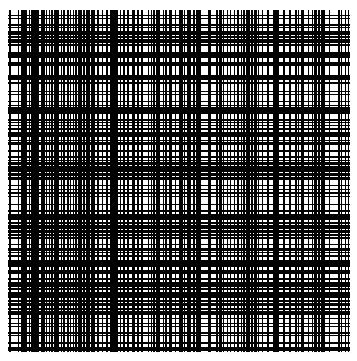
\includegraphics[width=0.5\linewidth]{pics/mask_256}
        \caption{\texttt{Nxm0} = 256}
        \label{fig:mask-256}
    \end{subfigure}%     
    \caption{Different separable masks generated with different \texttt{Nxm0}}
    \label{fig:sep_mask_multi}
    \end{figure}

\begin{figure}[ht]
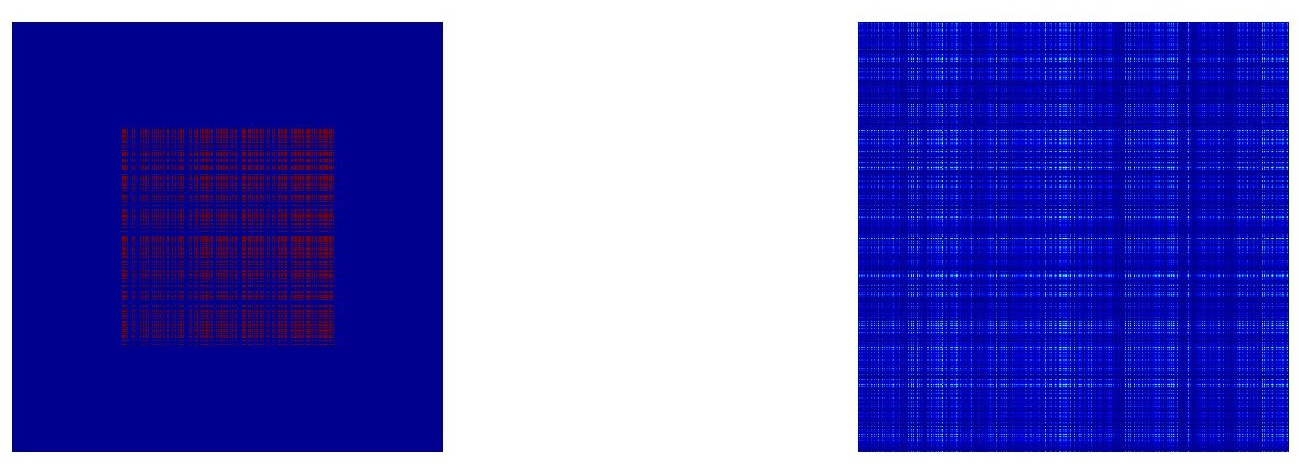
\includegraphics[width=\linewidth]{pics/diffracted_mask}
\caption{The mask on the left indicates undiffracted mask and the mask on the right indicates the diffracted separable mask}
\label{fig:diff_separable}
\end{figure}

It can be seen from Figure \ref{fig:rec_sep} that even in the presence of diffraction it would be possible to obtain reconstructions using equation \ref{eq:sep_final} by using a separable mask, unlike a non-separable mask which fails to provide any reconstruction in the presence of diffraction effects. 
  \begin{figure}[ht]
    \centering
    \begin{subfigure}{0.5\textwidth}
    \centering
        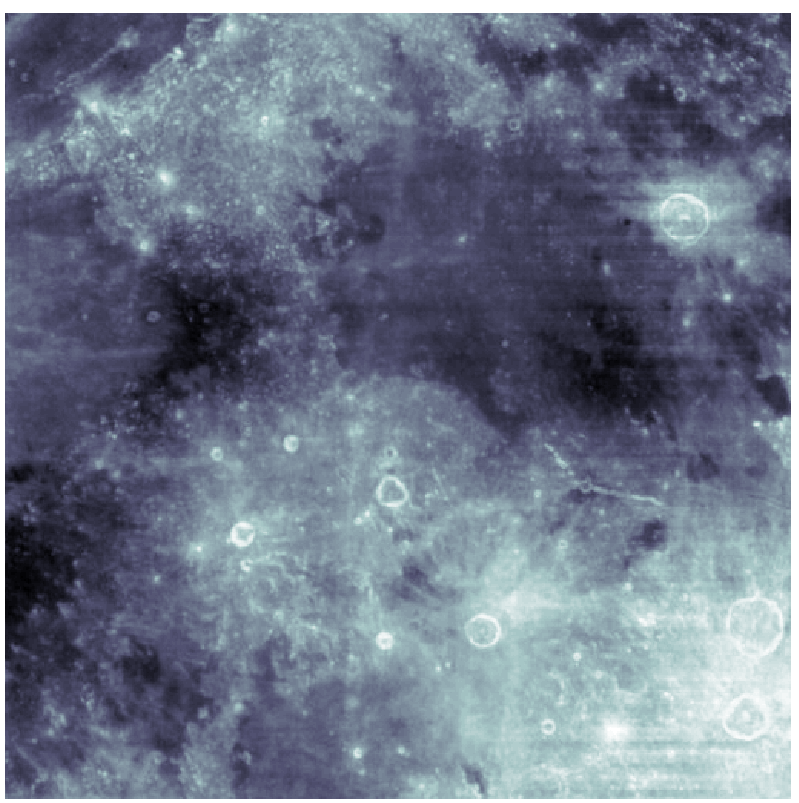
\includegraphics[scale = 0.25]{pics/sep_mask_rec}
    \end{subfigure}%
    \begin{subfigure}{0.5\textwidth}
    \hspace{4cm}    
    \centering
        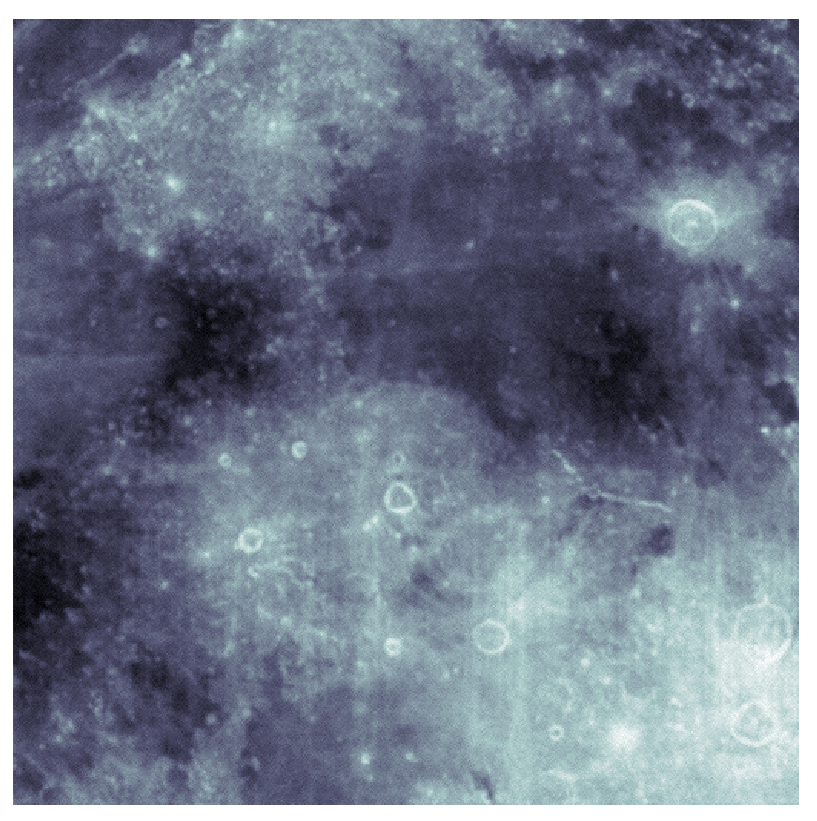
\includegraphics[scale= 0.25]{pics/sep_mask_rec_diff}
    \end{subfigure}
    \caption{The figure shows the reconstruction with and without fresnel diffraction effects for a separable mask using equation \ref{eq:sep_final}. We are able to obtain PSNR = 57.85 without diffraction effects. It can be seen that we can obtain reconstructions even in the presence of diffraction effects with PSNR = 57.93 }
    \label{fig:rec_sep}
    \end{figure}
It was seen that the separable mask would work best for our application and we can safely assume that we can use these masks to obtain reconstructions for extended object imaging in the visible light spectrum as the diffraction effects have also been taken into account.     
    
\chapter{Implementation}
In this chapter, we will be discussing the implementation of hardware and software of the camera that would be used for subsequent experiments.
The main specifications of the chosen cameras are shown in Table \ref{tbl:camera_specs}. These specifications are taken from the sensor data sheet and the camera manual provided by the vendors of the camera\cite{OV2640Arducam}\cite{OV5642Arducam}\cite{OV2640DS}\cite{OV5642DS}.  
\begin{table}[]
\centering
\caption{ Key Specifications Specifications of sensors Chosen}
\label{tbl:camera_specs}
\begin{tabular}{|c|c|c|}
\hline
Specification & OV2640 &  OV5642 \\
\hline
Voltage Level & 3.3/5V &  3.3/5V\\
 \hline
Frame Buffer Size & 384 KB & 8MB \\
 \hline
 Active Pixel Array Size& 1600$\times$1200&  2592$\times$1944 \\
 \hline  
 Camera Dimensions & 34mm $\times$ 24mm & 34mm $\times$24mm\\
 \hline
 Sensor Dimensions & 5725 $\mu$m $\times$ 6285 $\mu$m& 6945 $\mu$m $\times$ 6695 $\mu$m\\
 \hline
 Pixel Size & 2.2 $\mu$m $\times$ 2.2 $\mu$m & 1.4$\mu$m $\times$ 1.4 $\mu$m\\
 \hline
 Weight & 20 grams & 20 grams \\
 \hline
 Operating Temperatures & -10 to 55 degree celsius & -10 to 55 degree celsius \\
 \hline
 Electronic Interfaces Needed & SPI, I2C & SPI, I2C\\
 \hline
 Dynamic Range & 50 dB & 68 dB \\
 \hline
\end{tabular}
\end{table}
\section{Embedded Software of Camera}
One of the main reasons behind choosing the OV2640 and OV5642 CMOS sensors is that they already have a ready electronic interface that can be used to interface with standard 8-bit/16-bit microcontrollers. Arducam is an open source camera that comes along with open-source hardware and software that is needed to capture images using the CMOS sensor. Arducam is a platform that provides the hardware and software components necessary to interface OV2640 and OV5642 sensors with the conventional microcontroller platforms such as Arduino. One of the core components in every camera made by Arducam is that there is a component called Arduchip\cite{Arduchip}. It is a basically an Altera MAXII CPLD EPM240 processor that facilitates DMA memory transfer between the camera memory module and components such as microcontroller and thereby helping to reduce the development time for special applications such as space where the only computational resource that would be available are low power computing platforms such as microcontrollers with only synchronous serial interfaces such as I2C, SPI, etc. 

However, using the camera comes with its own advantages and disadvantages. The main advantage of using this platform is that the platform has open-source libraries that could be used to interface with ATMEGA328P, an 8-bit microcontroller. In space missions, it would not be possible to send high-powered microprocessors, and a microcontroller is used as an onboard computer. Arducam has standard software libraries that can be used to interface with Arduino making the cumbersome and lengthy job of writing an interface software to a CMOS sensor way more easier.  A disadvantage of the hardware module is the onboard memory that it has to capture an image. The OV2640 Arducam mini camera module can capture up to $1600 \times 1200$ resolution images with or without any form of compression. However, due to the limitation of the onboard OV2640 FIFO memory AL422B, it would be possible to capture only compressed images and not full resolution RAW images. The AL422B on-board FIFO has only 384KB of memory and that is not enough to obtain a full-resolution RAW image. One of the other disadvantages is that custom code needs to be written to obtain various controls that we need for our camera. We have to write our own camera control software if we need to control factors such as exposure time, ISO, etc. as the default software uses automatic exposure control to enhance the image quality. The camera module architecture is shown in Figure \ref{fig:arducam_arch}. The OV5642 offers a greater flexibility in terms of memory as it has a larger FIFO Buffer(8 MB).

 \begin{figure}[!htbp]
\centering
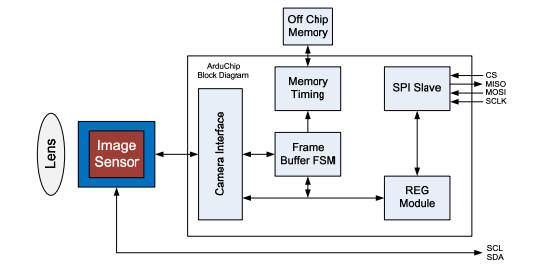
\includegraphics[scale=0.75]{pics/arducam_architecture}
\caption{Camera Architecture of Arducam Mini OV2640 Camera Module}
\label{fig:arducam_arch}
\end{figure}

The system for experiments is as shown in Figure \ref{fig:imp_setup}. The Arduino is connected to the camera module through an I2C interface. Using the I2c interface it possible to set registers that control the functioning of the camera such as the output format, digital signal processing, etc. SPI interface is used to transfer the image data from the camera module to the Arduino. The Arduino upon receiving the image data either writes it to an  SD card or sends it to the software on the PC through the USB connection. The software flow is shown in Figure \ref{fig:arducam_software}. We use the same software flow for both the CMOS sensors as the APIs are designed for use with many sensor models. The same set of libraries can be used for different CMOS sensors by simply adding some preprocessor directives to a \texttt{memorysaver.h} header file provided in the open-source library. To see the images on the PC, the vendor has provided a host PC software(not open source) and firmware which uses USB-UART to transfer images from the Arduino to PC. The firmware could be modified to ignore certain commands coming from the PC and using this we were able to modify the camera settings to our advantage. 
\begin{figure}[!htbp]
\centering

\includegraphics[scale=0.75]{pics/implementation_setup}
\caption{Implementation Setup}
\label{fig:imp_setup}
\end{figure}

One of the important factors that need to be controlled in camera is the exposure time. The Arducam libraries provide APIs for 10 different exposure levels for the OV5642 sensor. However, no such APIs are available for OV2640. Since OV2640 consumes lower power, it was decided to start the experiments with this camera. So, we need to write custom software to control the exposure level of this camera. The Arducam APIs used for the software are shown in Table \ref{fig:arducam_software}. The details of more APIs can be found in the software application notes\cite{ArducamSoftwareApp}. The default camera settings were used with only modifications to exposure in the case of OV2640 module. The CMOS sensor can be directly accessed using \texttt{wrSensorReg16\_8, wrSensorReg8\_8} functions which provide I2C bus access to the CMOS sensor.
\begin{figure}[!htbp]
\centering
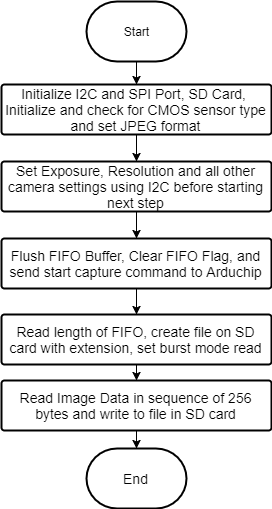
\includegraphics[scale  = 0.5]{pics/SoftwareFlowOV2640}
\caption{Software Flow used for image acquisition from CMOS sensors}
\label{fig:arducam_software}
\end{figure}


\begin{table}[ht]
\centering
\caption{ Details of Main APIs used}
\label{tbl:camera_apis}
\begin{tabular}{|c|c|c|}
\hline
API & Function \\
\hline
\texttt{InitCAM} & Initialize Camera Module\\
\hline
\texttt{set\_format} & \makecell{JPEG an BMP output formats \\can be selected}\\
\hline

\makecell{\texttt{clear\_fifo\_flag}\\ \texttt{read\_fifo\_length}\\
\texttt{set\_fifo\_burst} \\
\texttt{flush\_fifo}} & \makecell{These functions are \\used to control the FIFO buffer, \\read the size of \\the image  and \\to reset them when needed}  \\

\hline
\texttt{write\_reg} & \makecell{This function is used to write \\values to the specified register\\ address on the Arduchip.}\\
\hline
\texttt{\makecell{wrSensorReg16\_8\\wrSensorReg8\_8}} & \makecell{These functions are used to\\ set camera \\ registers using I2C. The first function \\ is used for 16-bit register\\ addresses and the \\second function is used for\\ 8-bit addresses}  \\
\hline
\texttt{\makecell{OV2640\_set\_JPEG\_size\\ \texttt{OV5642\_set\_JPEG\_size}}} & \makecell{These functions are used \\to set the resolution of the\\ output image } \\
\hline
\texttt{OV5642\_set\_Exposure\_level} & \makecell{This functions are used \\to set the exposure level of the \\OV5642 CMOS sensor}\\
\hline
\end{tabular}
\end{table}
\subsection{Exposure Control of OV2640}
In order to do experiments, it was required to control the exposure of the camera. In the default driver that was provided by the vendor, the exposure was automatically set using the Automatic Exposure Control (AEC) feature in the sensor. So, a modification was needed in the driver software. Fortunately, the driver is open source and there were libraries that could assist in setting the onboard registers through the I2C interface on the Arduino. First, let us have a look at how exposure control works in an OV2640 camera. All rolling shutter image sensors including OV2640 expose the sensor one-line at a time i.e. pixels in the same line are exposed at the same time and different pixels in different lines are exposed at a different time. So, the minimum exposure time would be one line time and the maximum exposure time would be the frame time. This is illustrated in Figure \ref{fig:RollingShutterOV2640}. By default, the pixel clock is set at 36MHz. We can calculate the minimum line time using the following equation:

$$
Minimum Exposure Time = 1/Pixel Clock * Pixel \ Clockes \ per \ line 
$$
As shown in Figure \ref{fig:ShutterTimingOV2640}, one line consists of 1922 pixel clocks(1600 for pixel data and 322 clocks of horizontal blanking). So the minimum exposure time would be 53.39$\mu$seconds and the maximum exposure time would be the frame time(multiply line time by 1200 + 44 lines of vertical blanking) which would be 66.63ms\cite{RollingShutterOV2640}. In order to control the exposure of the camera, it is necessary to modify registers of address 4, 10, 13, 45. So, these registers were modified according to the required exposure time value. The driver software on the Arduino was modified to obtain different exposure times.
\begin{figure}[ht]
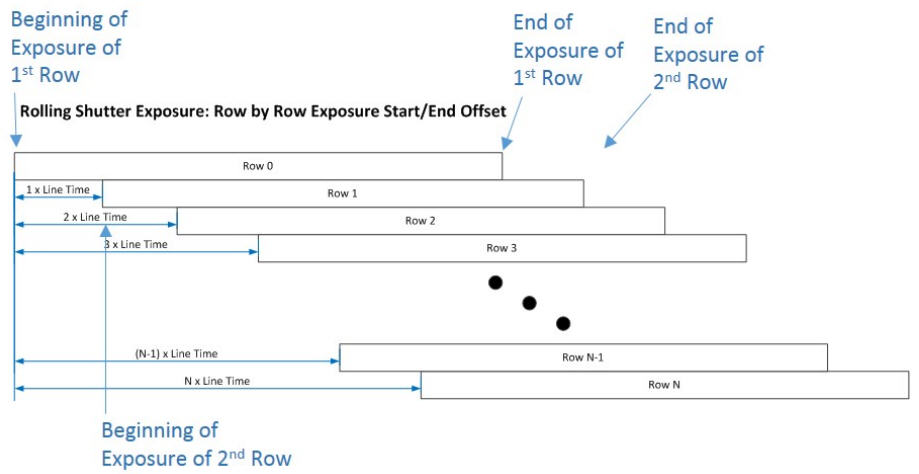
\includegraphics[width=\textwidth]{pics/rolling_shutter}
\caption{Rolling Shutter Operation on OV2640\cite{RollingShutterOV2640}}
\label{fig:RollingShutterOV2640}
\end{figure}

\begin{figure}[ht]
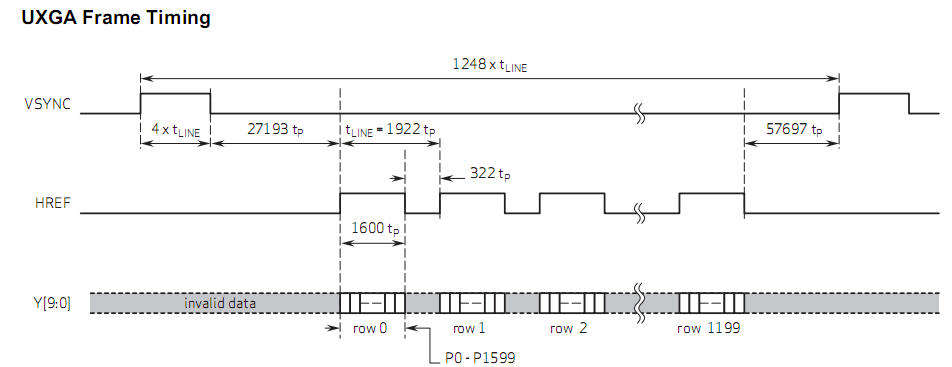
\includegraphics[width=\textwidth]{pics/OV2640timing}
\caption{Shutter Timing Diagram of OV2640\cite{RollingShutterOV2640}}
\label{fig:ShutterTimingOV2640}
\end{figure}

    \begin{figure}[ht]
    \centering
    \begin{subfigure}{0.5\textwidth}
    \centering
        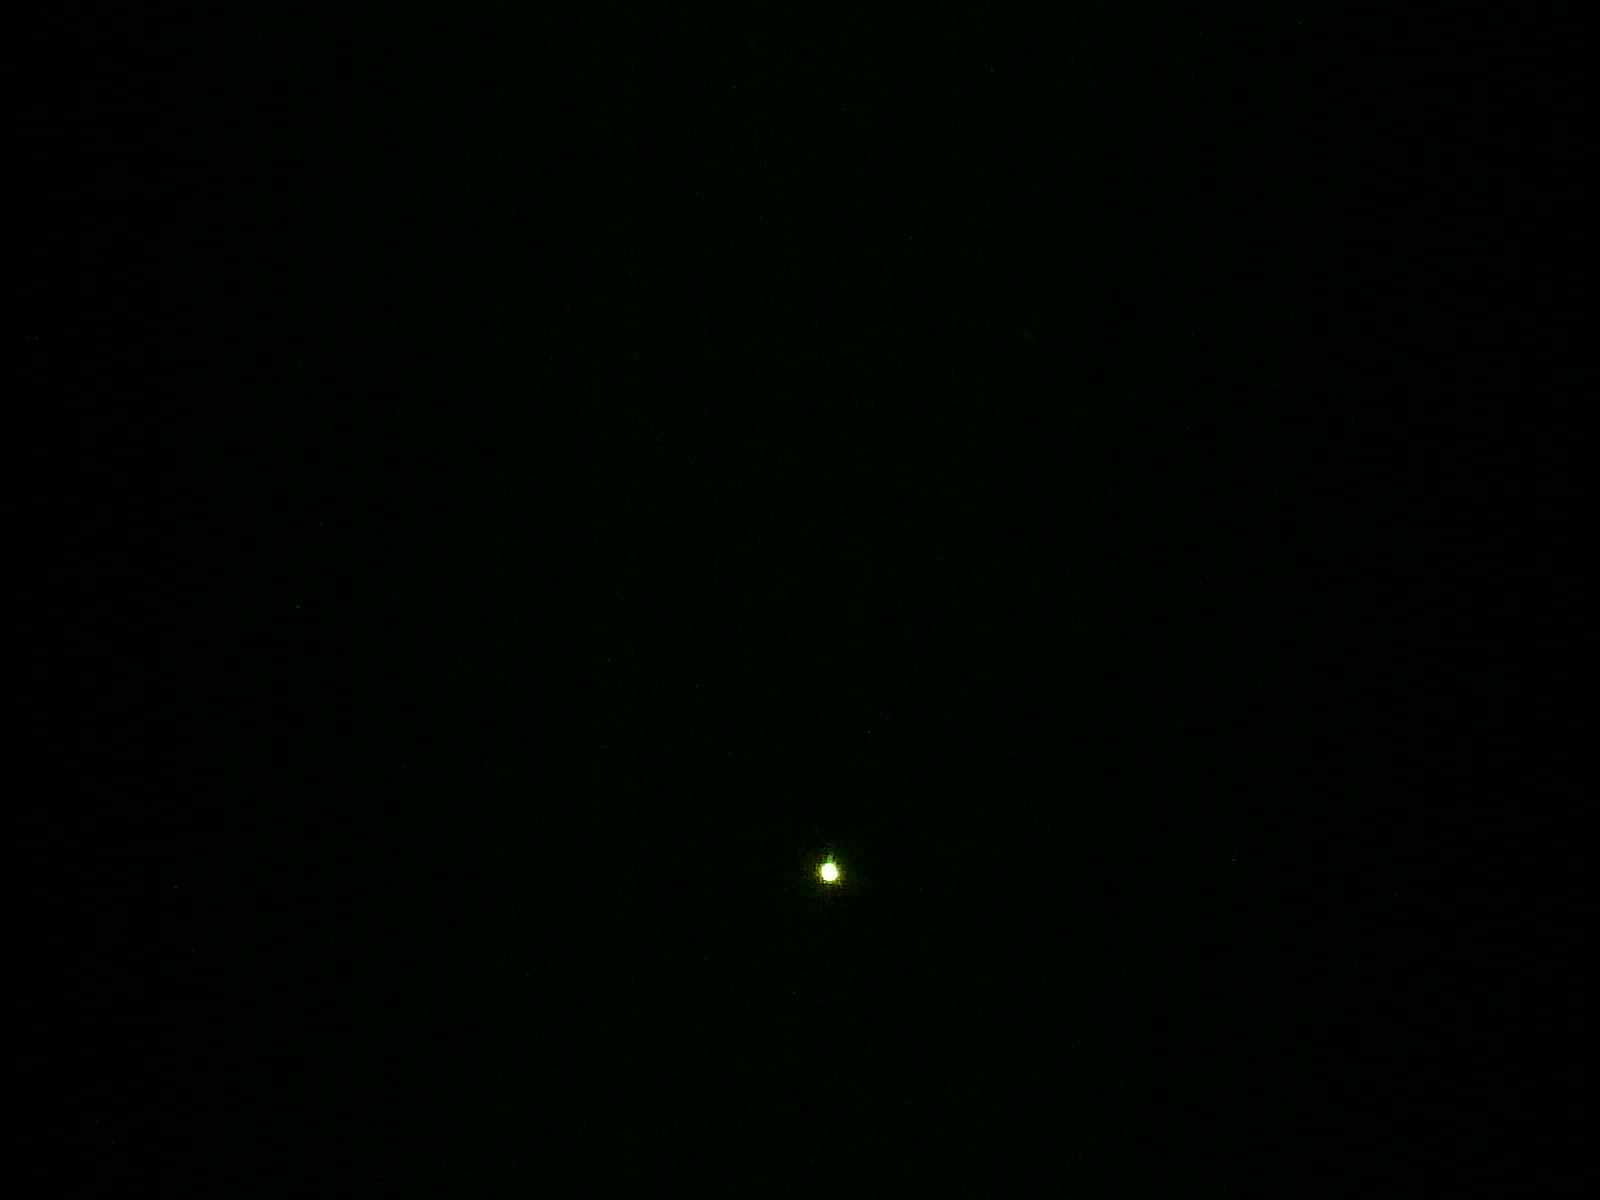
\includegraphics[width=0.5\linewidth]{pics/exposure/60us}
        \caption{60 $\mu$seconds}
        \label{fig:exp60us}
    \end{subfigure}%
    \begin{subfigure}{0.5\textwidth}
    \centering
        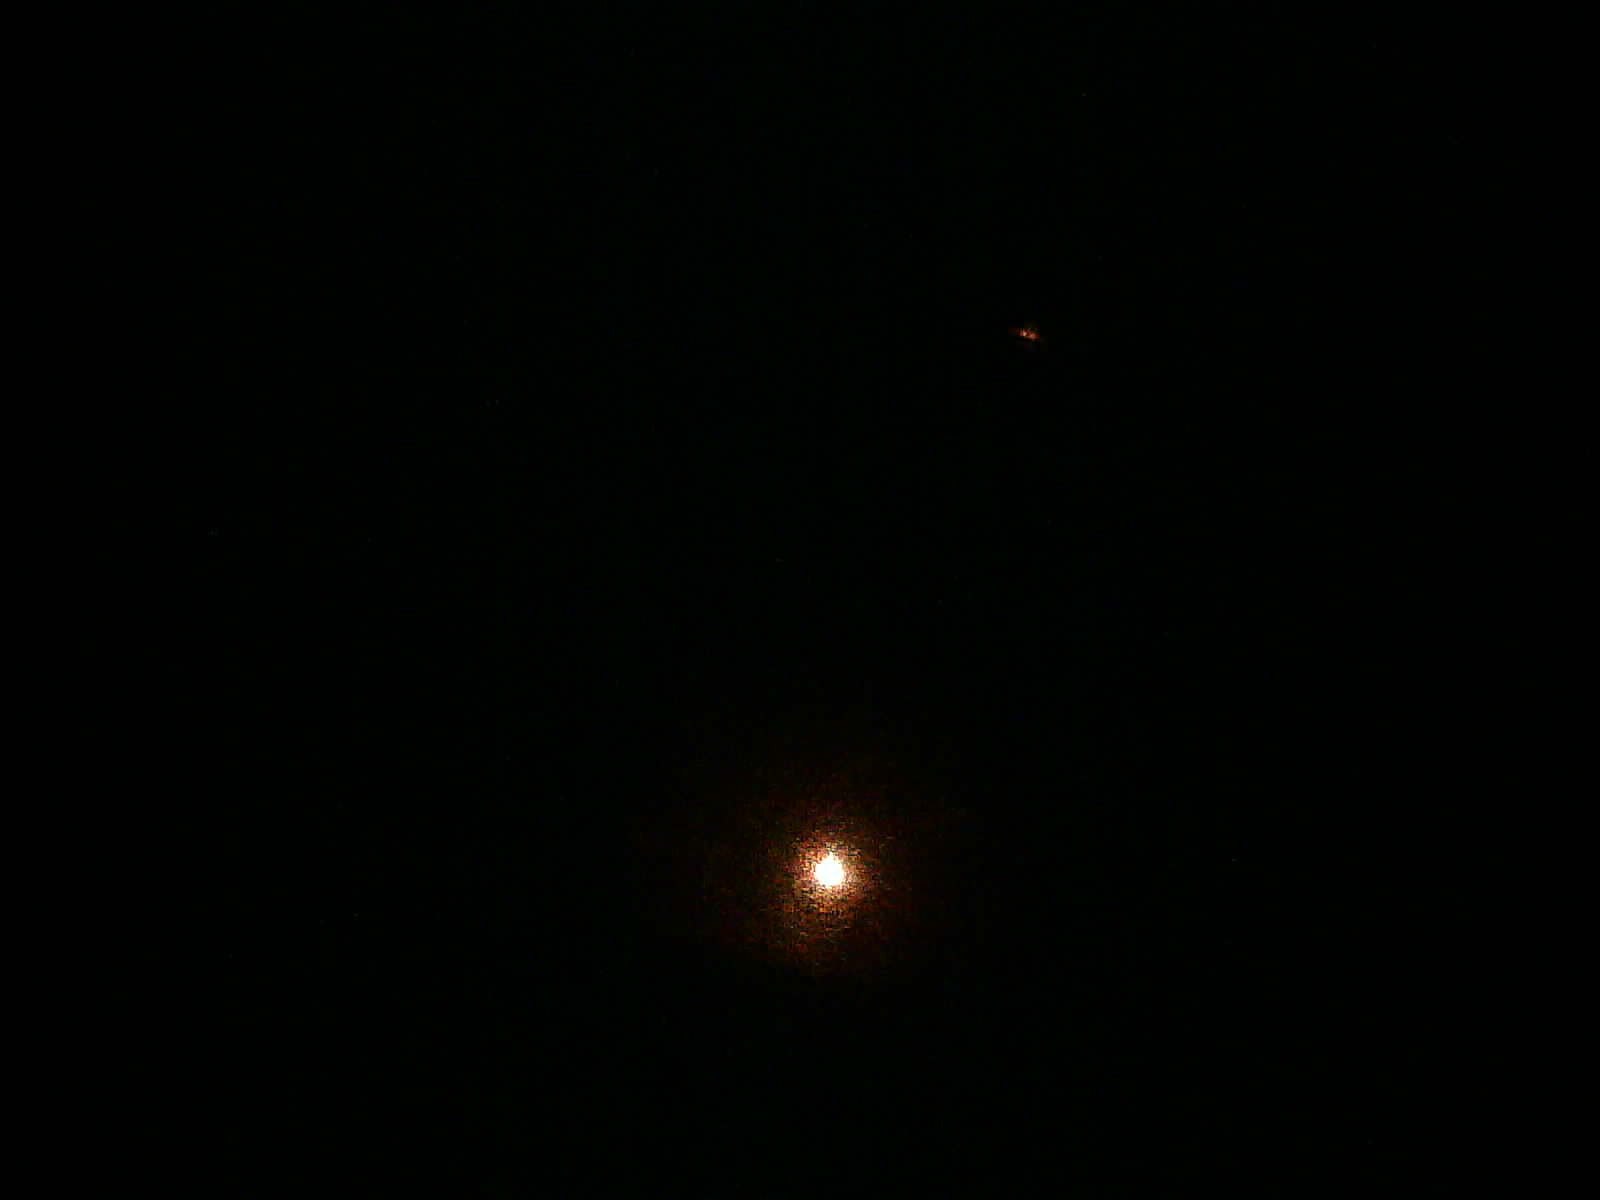
\includegraphics[width=0.5\linewidth]{pics/exposure/1ms}
        \caption{1ms}
        \label{fig:exp1ms}
    \end{subfigure}
    
    \begin{subfigure}{0.5\textwidth}
    \centering
        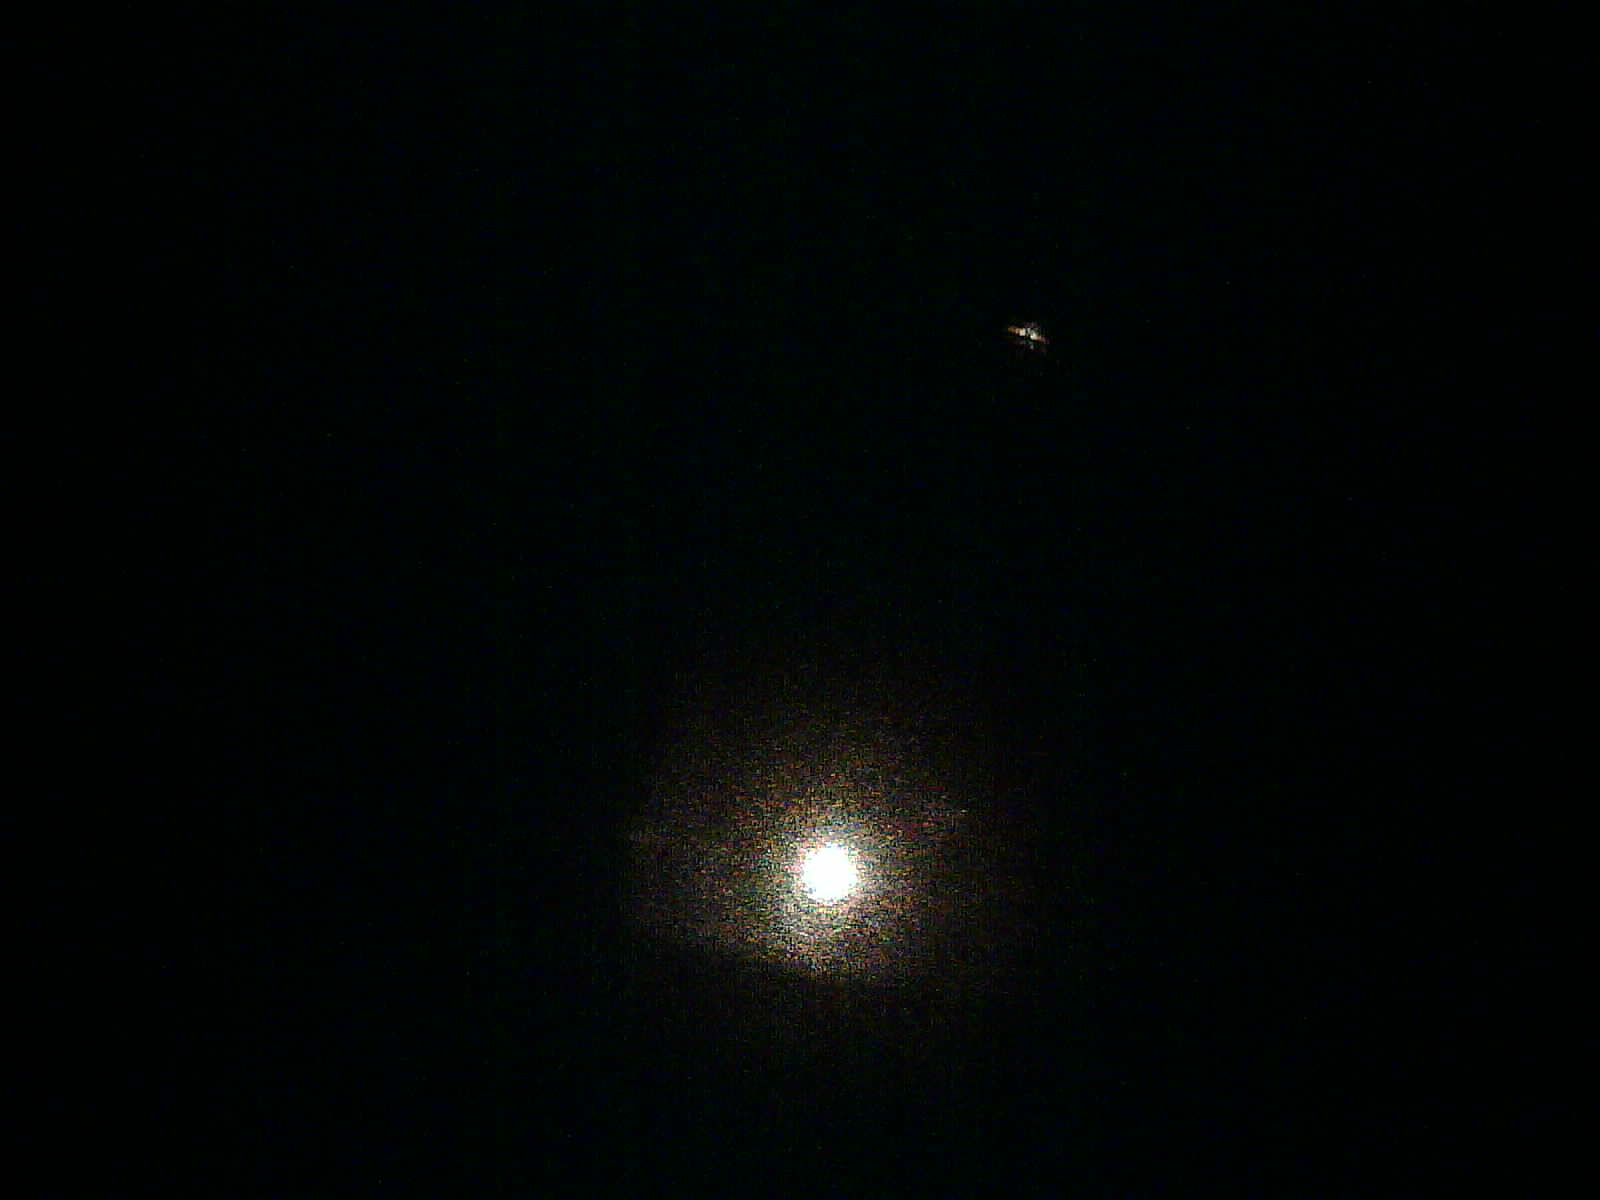
\includegraphics[width=0.5\linewidth]{pics/exposure/5ms}
        \caption{5ms}
        \label{fig:exp5ms}
    \end{subfigure}%
    \begin{subfigure}{0.5\textwidth}
    \centering
        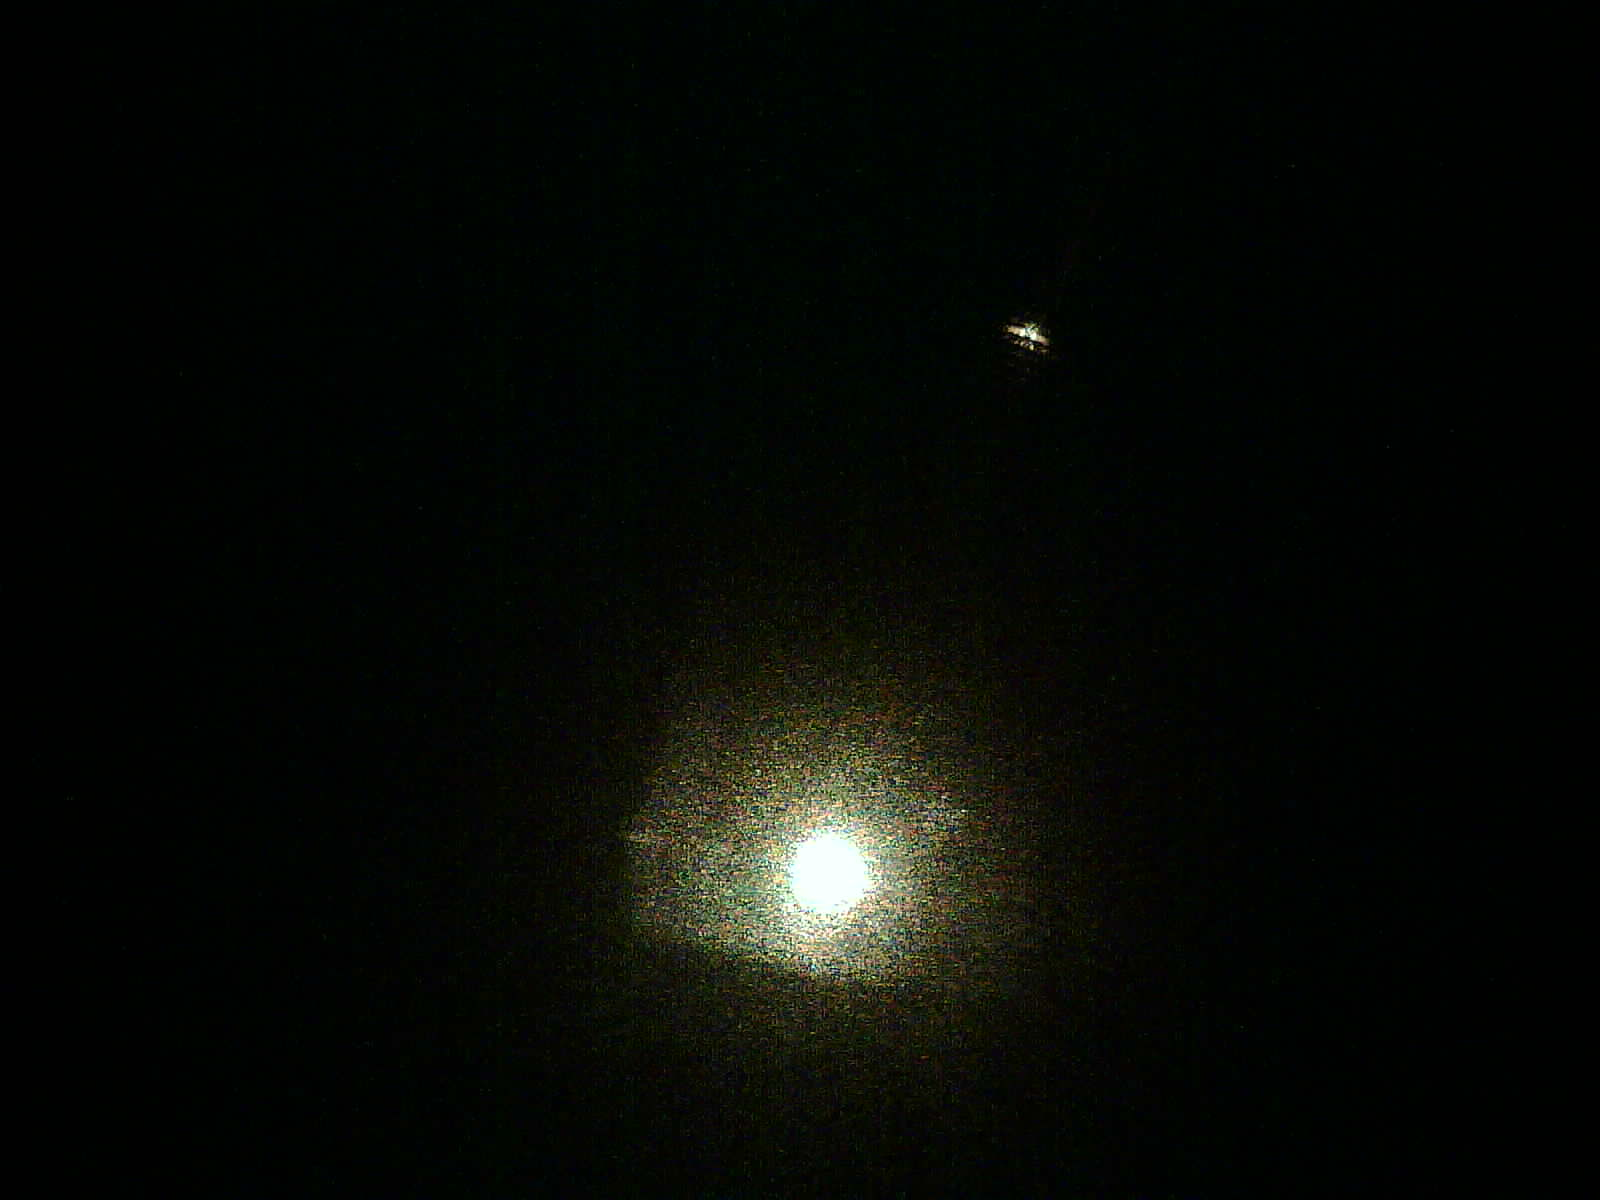
\includegraphics[width=0.5\linewidth]{pics/exposure/10ms}
        \caption{10ms}
        \label{fig:exp10ms}
    \end{subfigure}
        
        \begin{subfigure}{0.5\textwidth}
    \centering
        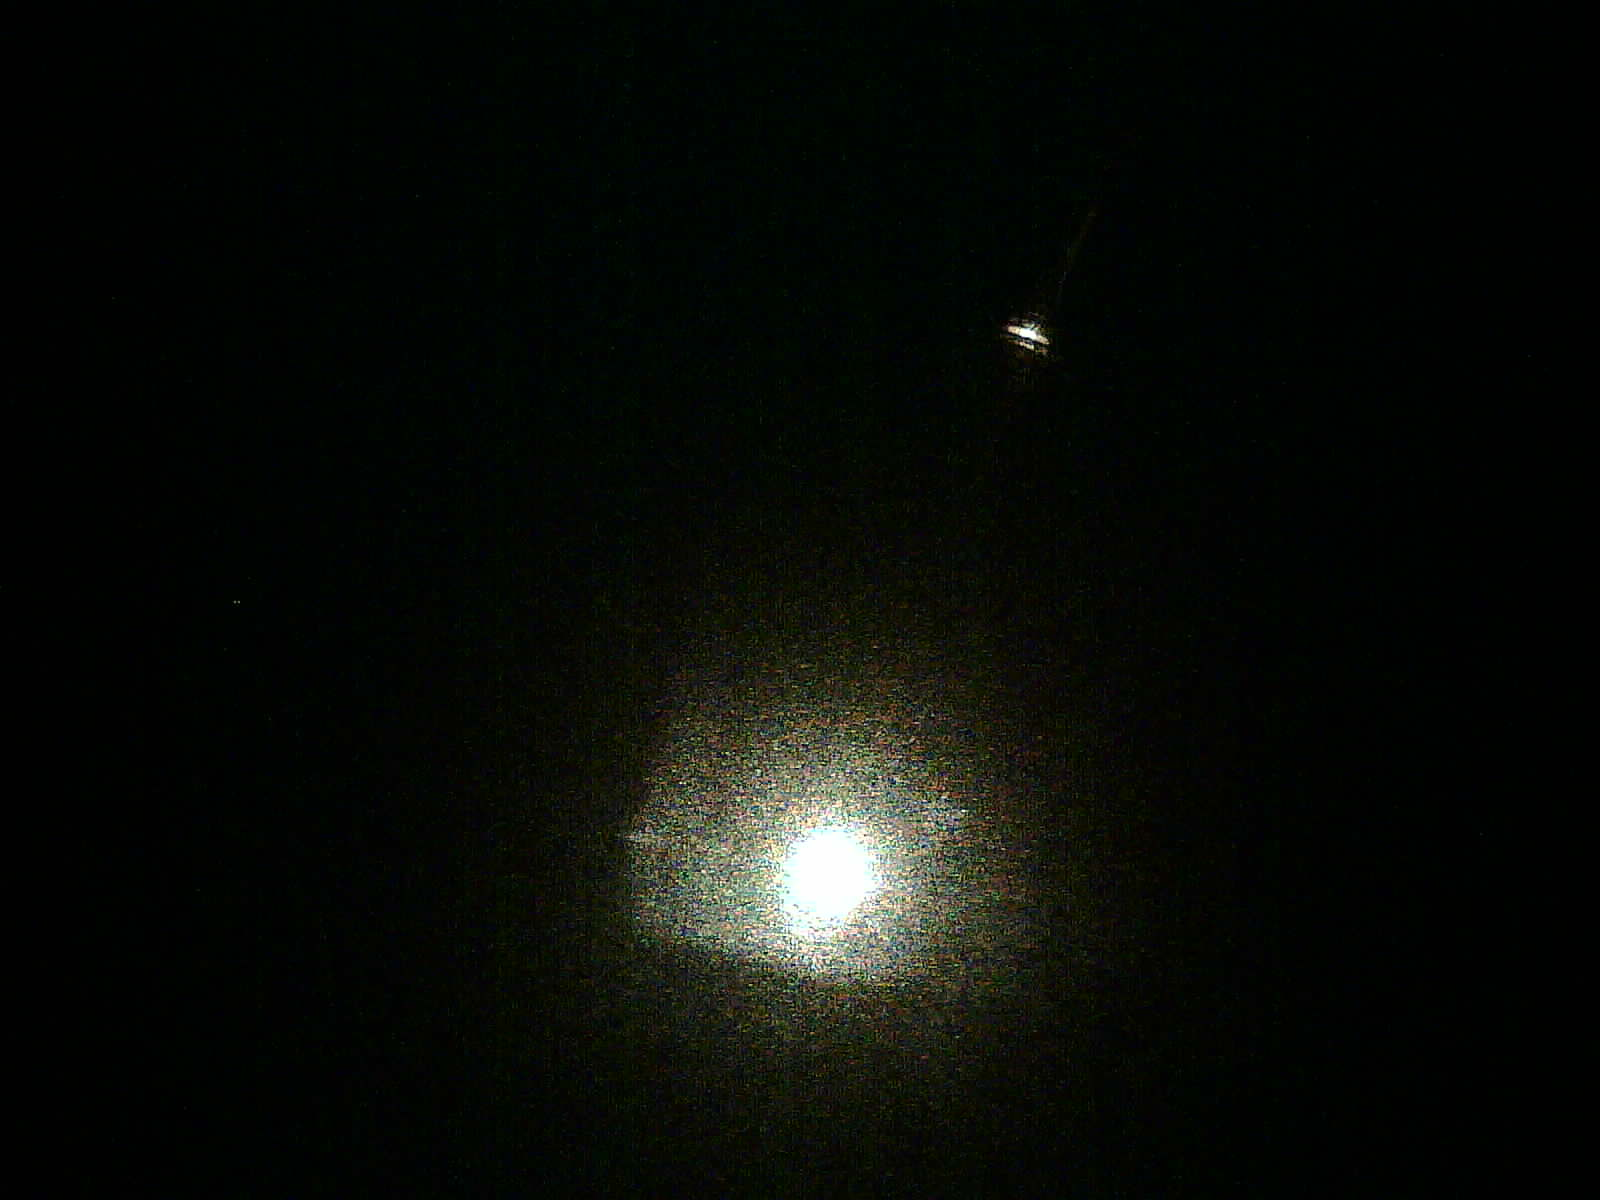
\includegraphics[width=0.5\linewidth]{pics/exposure/20ms}
        \caption{20ms}
        \label{fig:exp20ms}
    \end{subfigure}%
    \begin{subfigure}{0.5\textwidth}
    \centering
        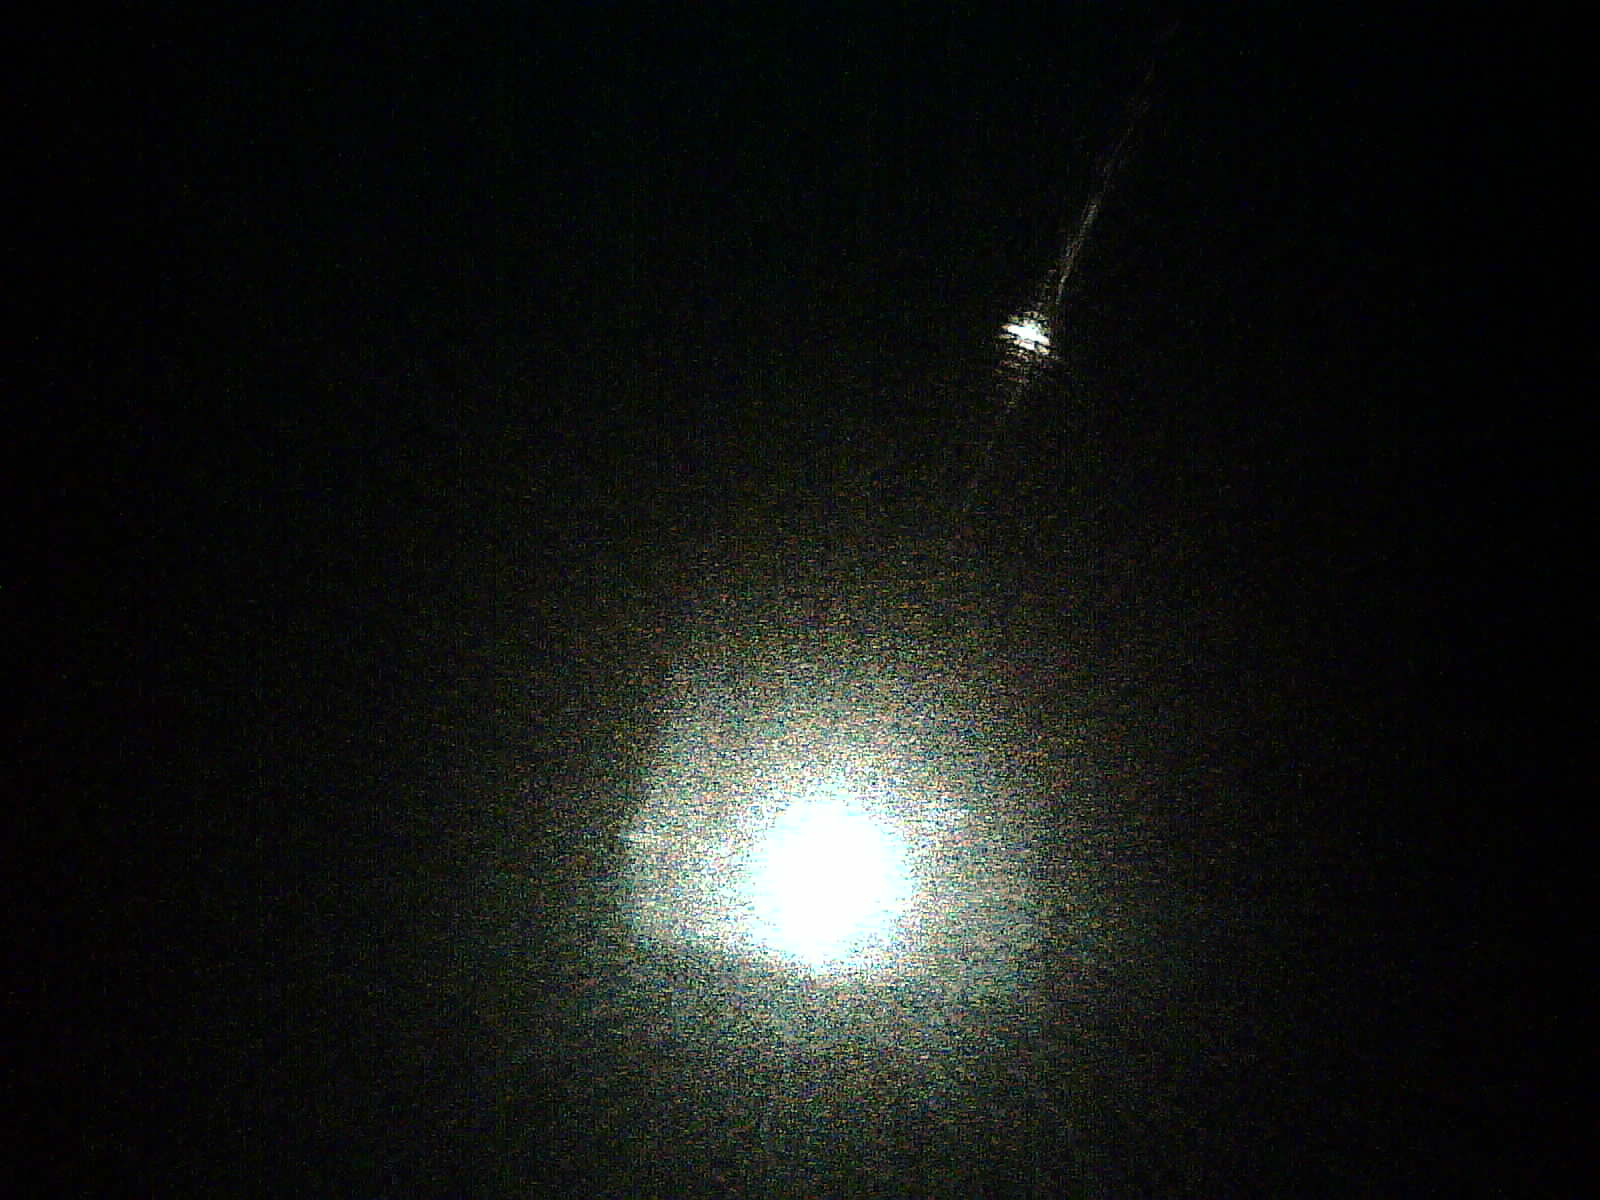
\includegraphics[width=0.5\linewidth]{pics/exposure/60ms}
        \caption{60ms}
        \label{fig:exp60ms}
        
    \end{subfigure}    
    \caption{Images of a laser beam caught in different exposure times(with lens)}
    \label{fig:exptests}
    \end{figure}
    
\section{Power Consumption of Sensors}
 One important aspect that also needs to be taken into account is the power consumption of the camera module(including the sensor, memory, voltage regulators, etc). Since, we have two camera modules, OV2640(low resolution, low power) and OV5642(high resolution, high power). The power consumption profile for OV2640 was provided by the manufacturer, however, the same is not available for OV5642. So, it was decided to perform power consumption measurements for the sensors manually. In order to find the amount of power consumed, we connect a 1 $\Omega$ resistor in series with the power line connecting the microcontroller and CMOS image sensor. The voltage measured across the resistor would be the current consumed by the camera sensors. The camera was operated in two modes: one in continuous "on" mode and the second mode was "on only when on". The second mode was activated clearing \texttt{GPIO\_PWDN\_MASK} when the camera is in use and set it once again once the camera is done taking the pictures and then saving it onto the memory card. The current consumption graph is shown in Figure \ref{fig:power}.
 
   \begin{figure}[ht]
    \centering
    \begin{subfigure}{\textwidth}
    \centering
        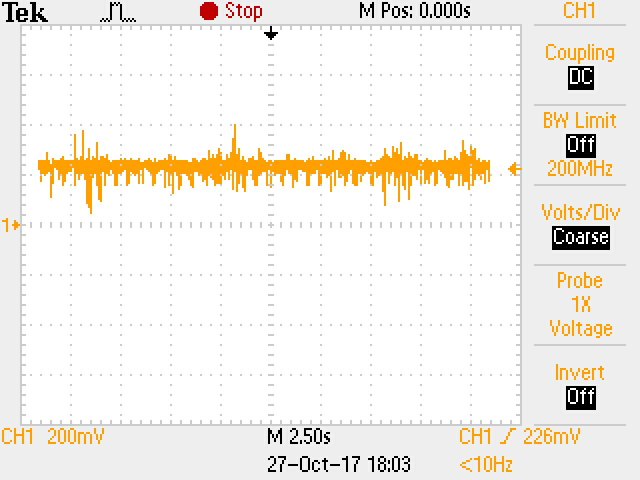
\includegraphics[width=1\linewidth]{pics/power_1.JPG}
        \caption{Voltage across  resistor when continuosly on}
    \end{subfigure}%
   
    \begin{subfigure}{\textwidth}
    \centering
        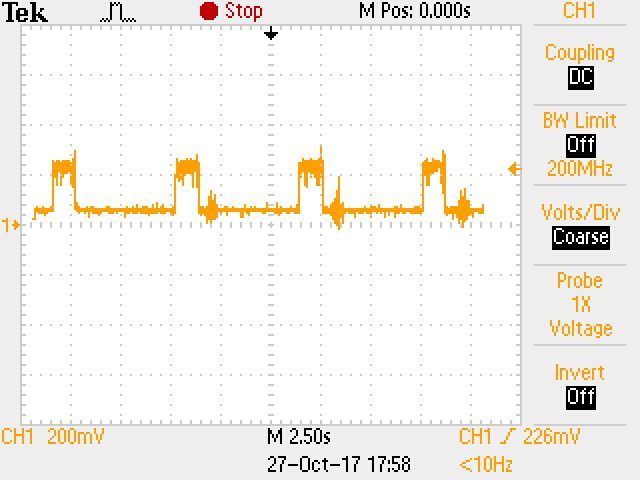
\includegraphics[width=1\linewidth]{pics/power_2.JPG}
        \caption{Voltage across  resistor when  using \texttt{GPIO\_PWDN\_MASK}}
    \end{subfigure}
       \caption{This figure shows the difference between keeping the OV5642 sensor module continuously on and using the \texttt{GPIO\_PWDN\_MASK}}
        \label{fig:power}
   \end{figure}
 
 It can be seen from Figure \ref{fig:power} that we can reduce power consumption by switching on the camera only when in use. The camera is operated in 5V mode. The current consumed by the camera is averaged  and the measured power consumption is shown in Table \ref{tbl:power_cons}. As expected, the higher resolution camera OV5642 consumes more power than OV2640. Since, OV2640 is consumes lower power and is also of lower resolution(which implies lesser size), we proceed to continue with the next set of experiments using OV2640.
\begin{table}[]
\centering
\caption{Measured power consumption of Cameras only when "on"}
\label{tbl:power_cons}
\begin{tabular}{|c|c|}
\hline
Sensor & Power \\
\hline
 OV2640 & 5V/93mA\\
 \hline
 OV5642 & 5V/233mA\\
 \hline
\end{tabular}
\end{table}
\chapter{Experimentations with SLM}
\label{chp:SLM}
\section{Initial Experiments to image mask}
I started off the experiment with the setup mentioned in the previous section. However, when trying to take an image of the mask with the CMOS sensor, I faced multiple challenges along the  way. The first challenge came in the form of the memory limitations of the camera module. The OV2640 camera module has only 384KB of memory which can store compressed JPEG images when imaging with lens. The memory limitation of the camera does not come into effect when imaging with lens as JPEG encoding is naturally designed for reducing size of real life artifacts and object scenes with a very high compression ratio. However, when using the same camera module, for lensless imaging, the size of the image easily exceeds the size of the FIFO buffer and the host software provided by the vendor is unable to read out the images. In order to overcome this challenge, I thought of increasing the extent of compression(with a trade-off of loss in quality) to image of the mask. This can be done by changing the \texttt{QSC} register(quantization scale factor) \cite{} of the CMOS sensor. The default value of the quantization scale factor is \texttt{0C}(hex value). This value was increased to \texttt{2F} by setting the registers using I2C as mentioned for the previous acceptance cone experiments. The size of the image was successfully reduced and the host software was able to read out images. After this the sensor was placed in front of the SLM and the experiments were continued. I started experimenting with the default masks provided by the SLM vendor before continuing onto the custom mask designed using simulations. The mask that was used was a binary axicon mask and binary mask which divides the SLM into two different halves.The figure of the mask is shown in Figure \ref{fig:InitMask}. The white portion of the horizontal mask is not visible.

After overcoming this challenge I faced the second challenge wherein, the mask was not visible and the central part of the sensor had saturated(whited out). This can be seen in Figure \ref{fig:InitMaskCMOS}. It can be seen from Figure \ref{fig:InitMaskCMOS} that the binary axicon mask is not at all visible due to the saturation of the CMOS sensor in the central region. The horizontal mask is imaged as a vertical mask by the CMOS sensor as the SLM is oriented vertically against the CMOS sensor. Even in the horizontal mask, the central portion has saturated. 

\begin{figure}[h]
    \centering
    \begin{subfigure}{0.5\textwidth}
    \centering
        
\includegraphics[width=0.5\linewidth]{pics/slm/binaryaxicon.png}
        \caption{Binary Axicon Mask}
        \label{fig:axiconmask}
    \end{subfigure}%
    \begin{subfigure}{0.5\textwidth}
    \centering
        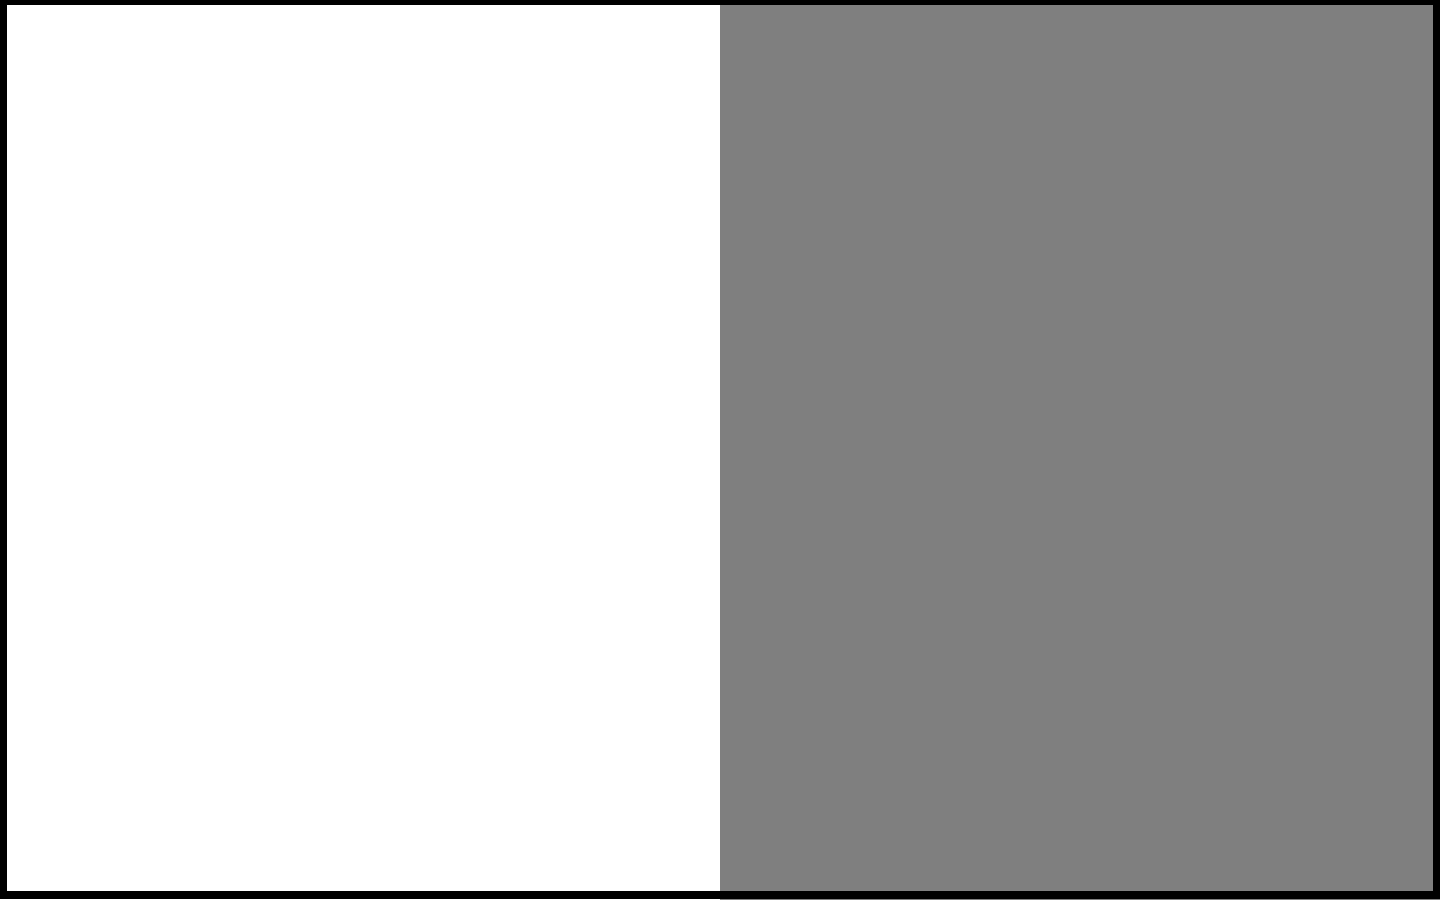
\includegraphics[width=0.5\linewidth]{pics/slm/hor-div.png}
        \caption{Horizontal dividable mask}
        \label{fig:hordivmask}
    \end{subfigure}
    \caption{Binary Masks used for Test}
    \label{fig:InitMask}
    \end{figure}
    
    \begin{figure}[h]
    \centering
    \begin{subfigure}{0.5\textwidth}
    \centering
        
\includegraphics[width=0.5\linewidth]{pics/slm/binaryaxiconcmos.jpg}
        \caption{Binary Axicon Mask imaged by CMOS}
        \label{fig:binaryaxiconcmos}
    \end{subfigure}%
    \begin{subfigure}{0.5\textwidth}
    \centering
        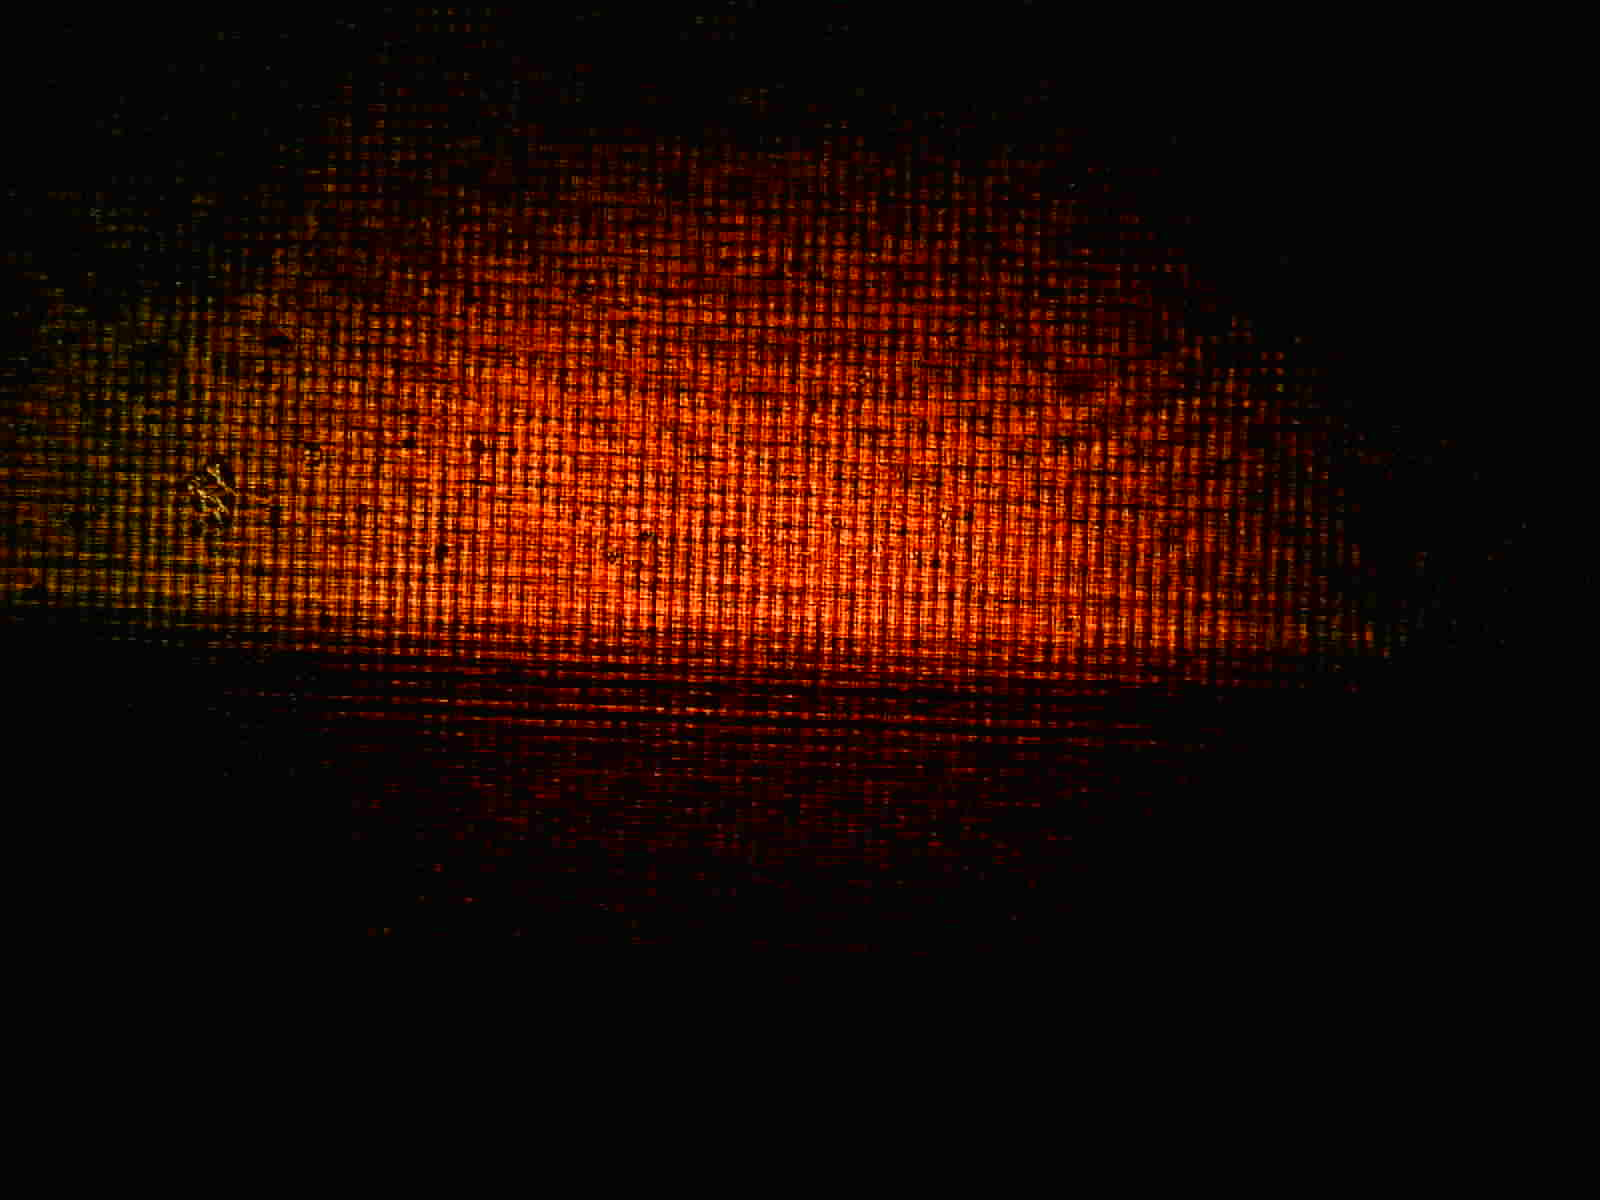
\includegraphics[width=0.5\linewidth]{pics/slm/horizontalcmos.jpg}
        \caption{Horizontal dividable mask imaged by CMOS}
        \label{fig:hordivmask}
    \end{subfigure}
    \caption{Binary Masks used for Test}
    \label{fig:InitMaskCMOS}
    \end{figure}
In order to solve these problems, multiple changes were made to the way the experiment was conducted. To avoid saturation, the exposure time of the CMOS sensor was reduced to the lease possible value(70 $\mu$seconds). Since, this did not affect the image of the mask formed on the sensor, it was decided to change the brightness and contrast levels of the SLM itself. The transmissive SLM acts as a screen and thus it has it's own brightness and contrast levels that affect the amount of light reaching the sensor. So, I decided to study the effect of the brightness and contrast on the image sensor. Also, two n.d filters were added to the setup that cut the intensity of light reaching the sensor by 75 percent. The SLM was placed approximately at a distance of 1 cm(10 mm) from the mask for these experiments.
\section{Effect of SLM brightness and contrast on CMOS sensor}
The first set of experiments was conducted to see the effect of brightness and contrast of the SLM on the image formed by the CMOS sensor. For this I thought of illuminating the CMOS sensor using the laser beam and then study the output image from the CMOS sensor for different gray levels on the CMOS sensor. Three gray levels(0,128,255) were chosen and the brightness/contrast levels were varied to see which brightness/contrast levels best represent the amount of light propotional to the grayness levels of the SLM. The brightness/contrast levels could be varied from 0 to 64 on the SLM. All the readings were normalized with respect to 255 to see how the intensity drops with respect to grayness levels. It can be seen from figures \ref{fig:slm_grayscale0},\ref{fig:slm_grayscale128},\ref{fig:slm_grayscale255} that there is a certain level of drop in intensity signal irrespective of the brightness levels. However, it is only in some gray levels that the drop is significant and noticeable(>25 percent reduction in intensity). The attenuation factors(ratio of reduction in intensity with respect to gray level 0) is plotted in tables \ref{tbl:attenuation128},\ref{tbl:attenuation255} that brightness levels and contrast levels close to 60 provide maximum attenuation in signals for graylevels 128(around 28 percent reduction) and gray levels 255(around 88 percent reduction) gray levels. It was decided to set the brightness and contrast values to 63 and study how the grayness level of the SLM affects the amount of light passing through the SLM.
\begin{figure}[h]
\centering
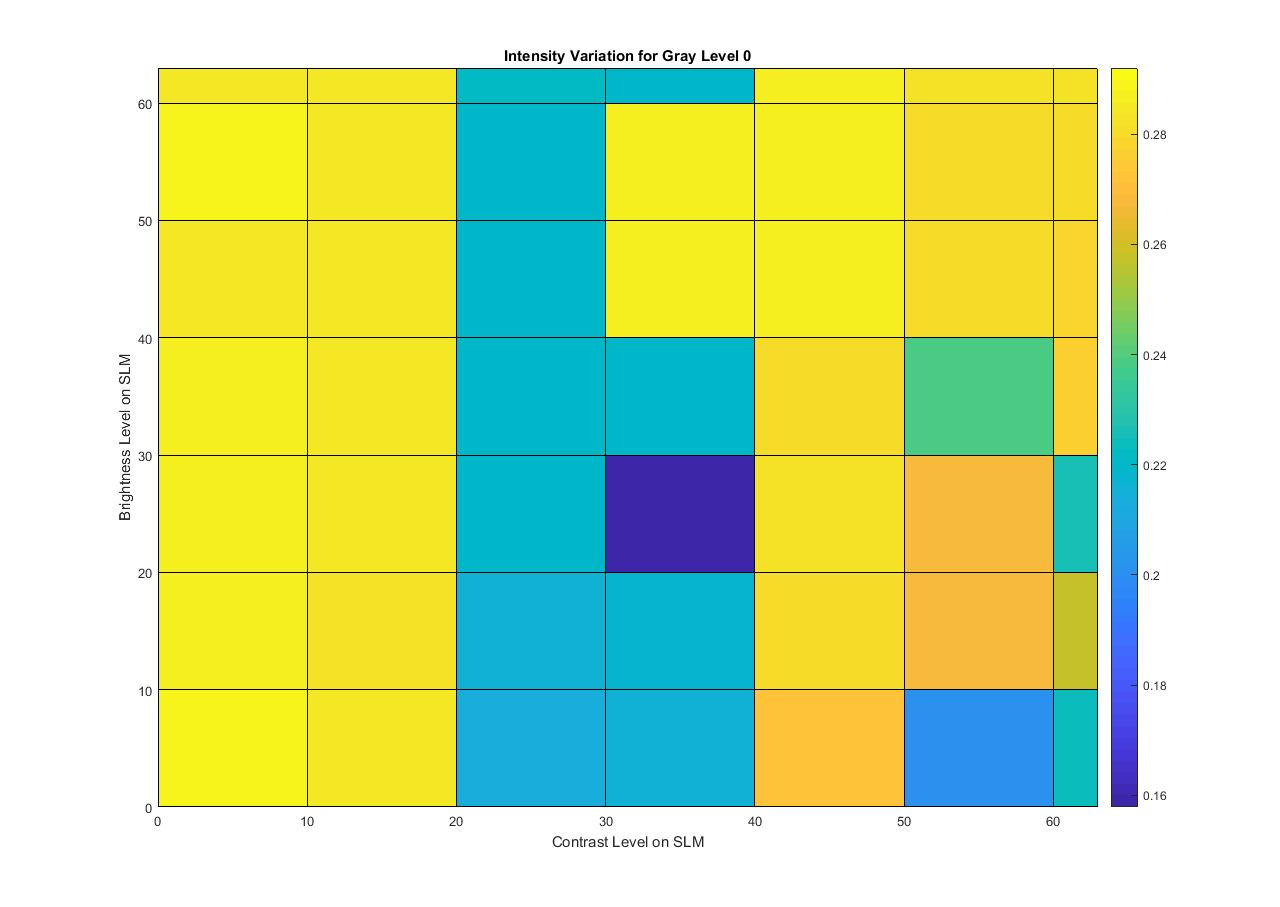
\includegraphics[scale=0.35]{pics/slm/slmgrayscale0.jpg}
\caption{Effect of brightness and contrast on intensity for grayscale 0}
\label{fig:slm_grayscale0}
\end{figure}
\begin{figure}[h]
\centering
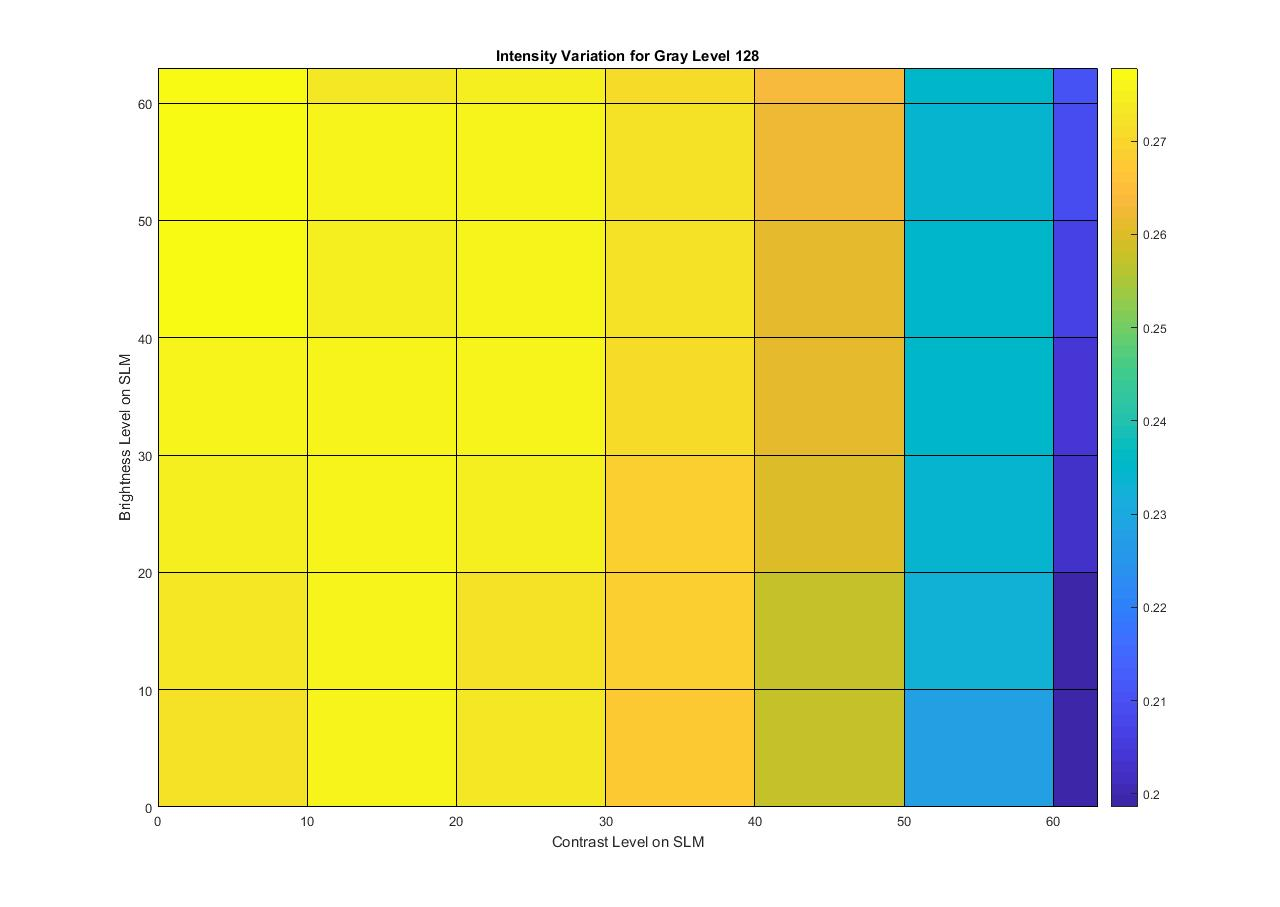
\includegraphics[scale=0.35]{pics/slm/slmgrayscale128.jpg}
\caption{Effect of brightness and contrast on intensity for grayscale 128}
\label{fig:slm_grayscale128}
\end{figure}

\begin{figure}[htbp]
\centering
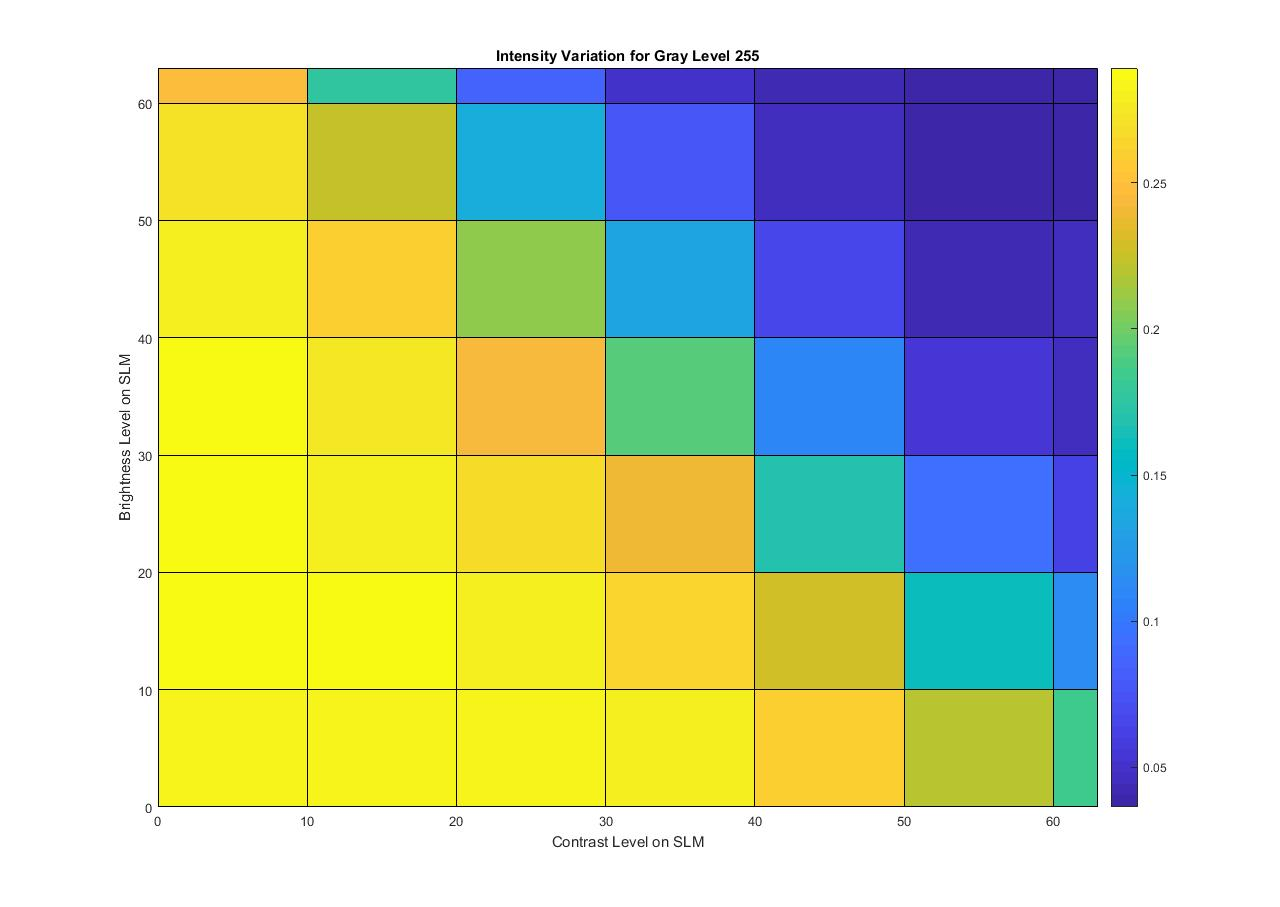
\includegraphics[scale=0.35]{pics/slm/slmgrayscale255.jpg}
\caption{Effect of brightness and contrast on intensity for grayscale 255}
\label{fig:slm_grayscale255}
\end{figure}

\begin{center}
\begin{table}[!h]
\begin{tabular}{|l|*{8}{c|}}\hline
\backslashbox{B}{C}
&\makebox[3em]{0}&\makebox[3em]{10}&\makebox[3em]{20}&\makebox[3em]{30}
&\makebox[3em]{40}&\makebox[3em]{50}&\makebox[3em]{60}&\makebox[3em]{63}\\\hline
\makebox[3em]{0} &0.9462&0.9669&1.2788&1.2455&0.9471&1.1301&0.8830&0.8875\\\hline
\makebox[3em]{10}&0.9537&0.9792&1.2639&1.2326&0.9206&0.8663&	0.7717&0.6853\\\hline
\makebox[3em]{20}& 0.9618&0.9717&1.2542&1.7043&0.9146&0.8726&0.8941&0.7327\\\hline
\makebox[3em]{30}&0.9622&0.9712&1.2600&1.2353&0.9266&0.9862&	0.7416&0.8852\\\hline
\makebox[3em]{40} &0.9731&0.9689&1.2625&0.9466&0.9127&0.8347&	0.7390&0.7205\\\hline
\makebox[3em]{50} &0.9593&0.9696&1.2597&0.9499&0.9145&0.8351&0.74525&0.7149\\\hline
\makebox[3em]{60} &0.9745&0.9634&1.2467&1.2331&0.9172&0.8288&	0.7433&0.7159\\\hline
\makebox[3em]{63}&0.9745&1.2669&1.233&1.2286&0.9121&0.8318&0.7394&0.7221\\\hline
\end{tabular}
\caption{Attenuation Factors of gray level 128 with respect to gray level 0 for different brightness and contrast levels}
\label{tbl:attenuation128}
\end{table}
\end{center}


\begin{center}
\begin{table}[!h]
\begin{tabular}{|l|*{8}{c|}}\hline
\backslashbox{B}{C}
&\makebox[3em]{0}&\makebox[3em]{10}&\makebox[3em]{20}&\makebox[3em]{30}
&\makebox[3em]{40}&\makebox[3em]{50}&\makebox[3em]{60}&\makebox[3em]{63}\\\hline
\makebox[3em]{0} &0.9834&0.9941&1.3247&1.2975&0.9602&1.0882&	0.81991&0.8124\\\hline
\makebox[3em]{10}&0.9971&1.0161&1.2988&1.2161&0.8096&0.5931&	0.4336&0.3780\\\hline
\makebox[3em]{20}& 1.011&0.9831&1.2162&1.5084&0.5896&0.3460&	0.2686&0.2113\\\hline
\makebox[3em]{30}&0.9966&0.9647&1.1133&0.8718&0.3898&0.2200&0.16253&0.1946\\\hline
\makebox[3em]{40} &0.9841&0.9138&0.9454&0.4592&0.2239&0.1554&0.1627&0.14317\\\hline
\makebox[3em]{50} &0.9350&0.7867&0.6462&0.2665&0.1593&0.1420&0.1296&0.1356\\\hline
\makebox[3em]{60} &0.8626&0.6265&0.3937&0.2237&0.1418&0.1345&0.1327&0.1291\\\hline
\makebox[3em]{63}&0.8188&0.7389&0.3334&0.2104&0.1375&0.1323&0.1385&0.1293\\\hline
\end{tabular}
\caption{Attenuation Factors of gray level 255 with respect to gray level 0 for different brightness and contrast levels}
\label{tbl:attenuation255}
\end{table}
\end{center}

\section{Effect of gray levels on CMOS sensor}
From the experimental results mentioned in the previous section, it can be seen that the maximum brightness and contrast levels of the SLM provide the maximum attenuation in signals. So, these values were chosen and the grayness levels of the SLM was varied from 0 to 255 and study how the grayness levels affect the amount of light passing through the SLM. The entire SLM screen is set to this grayness level so that the entire sensor is modulated with the same intensity of light.
The mean of the entire output image of the CMOS sensor is taken for plotting the signal and it is normalized with respect to the maximum reading and the graph is plotted. This is shown in figure \ref{fig:grayscale_slm_graph}. As it can be seen in the graph, the lowest point corresponds to an intensity reduction of approximately 88 percent. One important observation is that it is not possible to create a completely binary mask which blocks light as the maximum intensity reduction is only 88 percent. This will have an effect on the image reconstruction as it is assumed that the mask is completely binary. 

\begin{figure}[!htbp]
\centering
\includegraphics[scale=0.35]{pics/slm/grayscale_slm_graph.jpg}
\caption{Grayscale vs intensity of light received by the CMOS sensor.}
\label{fig:grayscale_slm_graph}
\end{figure}

\section{Imaging of Separable Mask using CMOS sensor}
In the previous section, we discussed how the SLM brightness and contrast affect the mask visibility on the CMOS sensor. In this section, we keep the mask brightness and contrast at maximum possible setting and image the mask. A random separable mask is generated for the resolution of the SLM. As mentioned in the previos sections, a random mask is one in which the row and column of the matrix can be expressed in the form:

$$
M = M_{x} * {M_{y}}^T
$$

Like in the simulations, a linearly spaced random vector is generated for a specific length(\texttt{Nxm0}) and interpolated to the SLM screen length(1024 X 768). Two vectors are generated(keeping \texttt{Nxm0} and \texttt{Nym0} constant) and the outer product of the vectors is taken to produce a mask that is same as the resolution of the SLM.
In order to make sure that the mask preserves the property of separability, we need to perform singular value decomposition on the output image from the CMOS sensor.

 Since the SLM is larger that the CMOS sensor, the sensor only images a particular portion of mask and not the complete mask itself.
The mask can decomposed into a singular matrix value no matter which part of the mask is imaged by the sensor. This was also verified in the MATLAB simulations. An example of doubly toeplitz mask generated is shown in figure \ref{fig:doubly_toepl_custom}. The region marked in red will also exhibit only one singular value on performing SVD.
\begin{figure}[h]
\centering
\includegraphics[scale=0.20]{pics/slm/mask_sub_prop.jpg}
\caption{Doubly Toeplitz mask}
\label{fig:doubly_toepl_custom}
\end{figure}
SVD forms the basis of the mask imaging experiment. We image the mask using OV2640 and see whether the mask still exhibits the same property when imaged by the CMOS sensor. The image of the doubly toeplitz mask imaged by OV2640 is shown in figure \ref{fig:dt_ov2640}.
\begin{figure}[h]
\centering
\includegraphics[scale=0.20]{pics/slm/ov2640dtmask.jpg}
\caption{Doubly Toeplitz mask imaged by OV2640}
\label{fig:dt_ov2640}
\end{figure}
As can be seen from the figure \ref{fig:dt_ov2640}, the OV2640 produces a very poor image of the mask. This can be attributed to the poor quality of compression. The quantization factor increased during the previous experiments in-order to reduce the size of the image has reduced the quality of the output image. Based on the mask image, we can be sure that it would be impossible to obtain proper reconstructions. So, it was decided to try whether other CMOS sensors would produce better quality pictures that would enable proper reconstruction. Based on the trade-off chosen previously, OV5642 sensor was also bought in-case of any failure. Since, OV2640 and OV5642 follow the same architecture and use the same open-source libraries, it was decided to check the image quality on OV5642. The OV5642 has an advantage that it has a bigger active sensor array(2592*1944) and comes with a larger FIFO buffer(8MB). In order to position these sensor on the stage, a script was written that would calculate the singular values in real time. The tilt of the sensor was adjusted such that the ratio of the first component to the second component is maximum. 
\begin{figure}[h]
\centering
\includegraphics[scale=0.125]{pics/slm/ov5642dtmask.jpg}
\caption{Doubly Toeplitz mask imaged by OV5642}
\label{fig:dt_ov5642}
\end{figure}
It can be seen from figure \ref{fig:dt_ov5642} that OV5642 produces a better image of the mask. In order to compare performance of OV5642, another web camera(Microsoft Lifecam HD 3000) was dis-assembled and the mask was imaged(See figure \ref{fig:dt_lifecam}). The difference in redness is due to the saturation level adjustment on LifeCam.
\begin{figure}[h]
\centering
\includegraphics[scale=0.25]{pics/slm/lifecamdtmask.png}
\caption{Doubly Toeplitz mask imaged by Microsoft Lifecam HD 3000}
\label{fig:dt_lifecam}
\end{figure}
A lot of methods were tried to increase the ratio of the first to the second singular value. Firstly, I tried to capture the image without any mask and capture the noise. I subtracted the noise from the mask image. However, this did not lead to any change in the singular component values. I then tried median filtering the output to reduce the gaussian noise effects and it increased the singular value ratio with all the CMOS sensors. This is shown in table \ref{tbl:dt_cmos_sensor_perf}. Table \ref{tbl:dt_cmos_sensor_perf} was plotted from the average of images in a particular data set using the same masks. The red channel data and the grayscale image data from the mask image are used for SVD. 
It can been from the table that OV2640 provides a better singular value ratio than OV5642. However, the highest singular component does not at all represent the mask that is programmed onto the SLM. So, OV2640 does not perform equivalent to OV5642 despite the higher ratio of singular component.
\begin{center}
\begin{table}[h]
\centering
\begin{tabular}{|l|*{4}{c|}}\hline
\backslashbox{Sensor}{Technique}&\makebox[4em]{SVD(Red)}&\makebox[10em]{SVD(Red) with filtering}&\makebox[4em]{SVD(Gray)}&\makebox[10em]{SVD(Gray) with filtering}\\\hline
\makebox[3em]{OV2640}&\makebox[3em]{7.833}&\makebox[3em]{11.16}&\makebox[3em]{8.05}&\makebox[3em]{10.49}\\\hline
\makebox[3em]{OV5642}&\makebox[3em]{8.74}&\makebox[3em]{10.84}&\makebox[3em]{7.04}&\makebox[3em]{10.78}\\\hline
\makebox[3em]{LifeCam}&\makebox[3em]{16.82}&\makebox[3em]{21.57}&\makebox[3em]{20.89}&\makebox[3em]{26.75}\\\hline
\end{tabular}
\caption{Performance of Different CMOS sensors(The values indicate the ratio of the first SVD to the second SVD value)}
\label{tbl:dt_cmos_sensor_perf}
\end{table}
\end{center}
The same results as in the simulation(only one singular value) could not be replicated because the mask that is produced by the SLM is not completely binary as observed in the previous experiment with SLM. If you observe the images from the sensor closely you can see that the black regions allow some portion of the light to pass through. This results in the image matrix becoming non-binary which in-turn results in secondary SVD components. One way to solve this would be to use a threshold and make the mask image binary but this would result in loss of diffraction and object data. Apart from this factor, another reason why other SVD components are observed is due to the presence of dead-pixel regions in the output data. The values of these pixels over-ride the values of the mask. These effects do not play a major role in lens based imaging but form a very important role in lensless imaging. Exposure plays a very important role in decomposability of the matrix. I first thought of increasing the exposure in-order to make the difference between the black and white more prominent (which in-turn increases separability). This idea seems to have worked out. The ratio of singular value to the exposure time is shown in Figure \ref{fig:svd_exposure}. The mask becomes separable as the exposure time is increased. However, this comes with a disadvantage. LifeCam has a very limited controllable range of exposure time and the sensor starts quickly saturating at around 2ms. When the sensor starts saturating, it leads to loss of data which in turn will have an effect on reconstruction. 
\begin{figure}[h]
\centering
\includegraphics[scale=0.35]{pics/slm/svd_graph_exposure.jpg}
\caption{Impact of Exposure Time on Singular Values}
\label{fig:svd_exposure}
\end{figure}
The best decomposition that I could get was using the LifeCam HD-3000 with exposure adjusted(without saturation) based on figure \ref{fig:svd_exposure}. The decomposition of mask into different components is shown in figure \ref{fig:svd_dec_exp}. 
\begin{figure}[ht]
\centering
\includegraphics[scale=0.50]{pics/slm/svd-decomp-exp.png}
\caption{Decomposition of best data set(Ratio of first to second component = 39.70 )}
\label{fig:svd_dec_exp}
\end{figure}
% CONCLUSIONS AND FUTURE WORK
\chapter{Conclusions and Future Work}
\label{chp:conclusionsandfuturework}

\section{Goals and Research Questions revisited}
In the beginning of the chapter, a research question and goals for the project were proposed. Now, let us revisit them to find out whether we have reached the goals of the project. The project was divided into these four sub-questions as given below:
\begin{itemize}
\item What would be the CMOS sensor that can be used for the camera? 
In chapter 2 of this report, the survey of CMOS sensors that have been used in previous CubeSat missions has been conducted. Based on various factors, OV2640 and OV5642 were chosen. This also indicates the achievement of the first goal.
\item How do we design the hardware and software for such a camera that can be used in Delfi-PQ satellite?\\
The main factor in choosing OV2640 and OV5642 was the presence of open source libraries,  and open source electronic interface hardware. The software and the hardware mechanism for controlling the cameras have been described in Chapter 4 of the report. All the experiments described in the later chapters of the report were developed using the same hardware and software described in Chapter 4. This also indicates the achievement of the second goal.
\item What would be the field-of-view and spatial resolution of the lensless camera?\\
An experimental setup to determine the acceptance cone of the CMOS sensor has been devised. The experimental results were incorporated into the previously completed simulations. Based on the experimental results, OV2640 had an acceptance angle of 43.6 degrees. It was found that the field of view of the lensless system had reduced 38 percent and 31.8 percent in the horizontal and vertical directions compared to a conventional lens-based system. The effective area of the sensor that could be used also reduced by 52 percent. The spatial resolution of the designed camera was calculated and the entire procedure for calculating the spatial resolution is described in Chapter 2 and Chapter 5 of the report. This also indicates the achievement of the third goal.
\item What would be the computational algorithm that would be used in such a lens-less camera? How do we experimentally prove the concept of lens-less imaging?\\
The computational algorithm mainly depends on the mask that we use for imaging. Two kinds of masks were evaluated namely, separable and non-separable masks. It was found that non-separable masks cannot be used to image objects in the visible light spectrum using existing computational methods available in the literature. So, we decided to go for a separable Toeplitz mask. It was found in the simulations that separable Doubly-Toeplitz mask could be used to reconstruct objects even in the presence of diffraction effects. The entire simulation workflow is described in Chapter 3 of the report.

Experimental verification of lensless imaging required multiple stages of experiments. After determining the field of view of the OV2640 sensor, the imaging of the separable mask was tried using OV2640. However, it was found out that OV2640 could not be used due to the limitation of the onboard FIFO buffer of the camera. Because of this, we decided to use OV5642 which has a bigger FIFO buffer. OV5642 is able to image the mask perfectly and preserves the separable property of the mask. The entire experimental approach was done using singular value decomposition and is mentioned in Chapter 6 of the report.  

The next step was to determine the system matrices of the lensless camera. To do this, we decide to use a Hadamard basis matrix as it could provide enough amount of light to produce a measurable sensor response. Using a basis matrix also provided better reconstruction and preserved the original object property as seen in the simulation results. This method requires us to use $2N$ calibration patterns on the LCD if we want to reconstruct images of resolution $N \times N$. This method was not verified experimentally and forms the final step of proving the concept of lensless imaging experimentally. The strategy and scheme for achieving this are described in Chapter 7 of the report. This indicates that there is some more experimental verification required to achieve the final goal.

\end{itemize}

Now, let us come to the main research question:
\textbf{Is it possible to design ``lensless coded" aperture cameras with a small form-factor(thickness $<$ 10mm) using COTS(commercial off-the-shelf) components that can be used in U-class Spacecraft ?}\\
The experimental results with commercially available camera modules OV2640 and OV5642 provide a good insight into the lensless imaging methodologies. The previous studies done in this field did not have any memory limitations like we faced with OV2640. The camera with bigger memory such as OV5642 could retain the properties of the mask when we experimentally tested them. A separable scene on the outside also yields a separable scene on the CMOS sensor. A scheme for determining the system matrices of a lensless imaging system is designed and simulated. However, the experimental determination of this scheme has not yet been verified. The simulations and experiments done in this work provide a good picture and insight into the concept of lensless imaging as a whole. The experimental results achieved till now indicate that commercially available cameras can be used but more experiments need to be performed before this question can be answered with more certainty. 

\section{Future Work}
There is a great scope for developing the work mentioned in this thesis. This work can be improved and extended in the following ways:
\begin{itemize}
\item Experimental determination of System Matrices: A scheme for experimental determination of the system matrix has been described in Chapter 7 of the report. This needs to be completed to completely realize the concept of lensless imaging. The scheme described is extremely time consuming as it requires $2N$ measurements(one-time procedure) to perform complete reconstructions for $N \times N$ resolution images. This scheme can also be improved to reduce the number of measurements needed to accurately estimate the system matrices. 

\item Fabrication with masks: This work uses transmissive Spatial light modulators(SLM) to simulate the effects of a mask. It was observed that a complete binary mask cannot be achieved with this equipment. Lithographic photomasks can be fabricated and can offer better performance than using an SLM.

\item Improving the computational method for reconstruction: This work uses regularization along with inversion to perform reconstructions. This method can also be improved using other methods to denoise the reconstruction such as SVD, BM3D and total variation based methods\cite{Flatcam}. These methods could be tried out on the existing simulations and studied whether they provide better reconstructions.

\item Hardware Improvements: OV2640 could not be used due to the limited onboard memory. The future work can also look into improving the camera hardware by replacing the memory of the camera module. This would also require a change in the hardware/software implementations of the library. Arducam can be contacted on how to achieve this. Also, they release improved versions of the camera modules every year.
\end{itemize}



% BIBLIOGRAPHY
%#define SORTED 1
\bibliographystyle{../bib/latex8}
\bibliography{../bib/mycollection}

%\appendix

%\begin{appendices}
\section*{Appendix A Camera Dimensions}
This section shows the dimension of the camera module as provided by the camera vendor.

\begin{figure}[!htbp]
\centering
\includegraphics[width = 0.75 \linewidth]{pics/arducam_mech}
\caption{Dimensions of both OV5642 and OV2640 camera modules}
\label{fig:arducam_mech}
\end{figure}

\end{appendices}

\end{document}

